\documentclass{ximera}

\input{../../../preamble.tex}


\definecolor{fvdnavy}{HTML}{071D43}
\definecolor{fvdcyan}{HTML}{20BFC6}
\definecolor{fvdcyanlight}{HTML}{EFFCFB}
\definecolor{fvdmagenta}{HTML}{F10D69}
\definecolor{fvdmagentalight}{HTML}{FFF1F7}
\definecolor{fvdtext}{HTML}{163044}





%=================================================
% Pedagogische omgevingen
% PDF: tcolorbox
% HTML: learning-box
%=================================================

\newenvironment{voorkennis}
{%
    \ifdefined\HCode
        \HCode{%
<section class="learning-box learning-box--prior">
<div class="learning-box__header">
<span class="learning-box__icon" aria-hidden="true"></span>
<span class="learning-box__title">Voorkennis</span>
</div>
<div class="learning-box__content">
        }%
        \begin{itemize}
    \else
       \begin{tcolorbox}[
    enhanced,
    breakable,
    colback=fvdcyanlight,
    colframe=fvdcyan,
    coltext=fvdtext,
    boxrule=0.5pt,
    leftrule=4pt,
    arc=4mm,
    outer arc=4mm,
    left=7mm,
    right=6mm,
    top=5mm,
    bottom=5mm,
    before skip=6mm,
    after skip=6mm,
    title=Voorkennis,
    coltitle=fvdcyan,
    fonttitle=\bfseries\Large,
    attach title to upper={\par\smallskip},
    boxed title style={
        empty,
        left=0mm,
        right=0mm,
        top=0mm,
        bottom=0mm
    },
    overlay={
        \draw[
            fvdcyan,
            line width=0.5pt
        ]
        ([xshift=42mm,yshift=-13mm]frame.north west)
        --
        ([xshift=-7mm,yshift=-13mm]frame.north east);
    }
]
        \begin{itemize}
    \fi
}
{%
    \end{itemize}
    \ifdefined\HCode
        \HCode{%
</div>
</section>
        }%
    \else
        \end{tcolorbox}
    \fi
}


\newenvironment{leerdoelen}
{%
    \ifdefined\HCode
        \HCode{%
<section class="learning-box learning-box--goals">
<div class="learning-box__header">
<span class="learning-box__icon" aria-hidden="true"></span>
<span class="learning-box__title">Leerdoelen</span>
</div>
<div class="learning-box__content">
        }%
        \begin{itemize}
    \else
\begin{tcolorbox}[
    enhanced,
    breakable,
    colback=fvdmagentalight,
    colframe=fvdmagenta,
    coltext=fvdtext,
    boxrule=0.5pt,
    leftrule=4pt,
    arc=4mm,
    outer arc=4mm,
    left=7mm,
    right=6mm,
    top=5mm,
    bottom=5mm,
    before skip=6mm,
    after skip=6mm,
    title=Leerdoelen,
    coltitle=fvdmagenta,
    fonttitle=\bfseries\Large,
    attach title to upper={\par\smallskip},
    boxed title style={
        empty,
        left=0mm,
        right=0mm,
        top=0mm,
        bottom=0mm
    },
    overlay={
        \draw[
            fvdmagenta,
            line width=0.5pt
        ]
        ([xshift=42mm,yshift=-13mm]frame.north west)
        --
        ([xshift=-7mm,yshift=-13mm]frame.north east);
    }
]
        \begin{itemize}
    \fi
}
{%
    \end{itemize}
    \ifdefined\HCode
        \HCode{%
</div>
</section>
        }%
    \else
        \end{tcolorbox}
    \fi
}


\addPrintStyle{../../..}

\title{Gravitatie: aantrekking op afstand}
\author{Ingmar Herreman}

\begin{abstract}
Waarom valt een appel naar de aarde? Waarom blijft de maan in de buurt
van de aarde? En waarom bewegen planeten rond de zon?

Op het eerste gezicht lijken dit verschillende verschijnselen. Newton
zag echter dat ze met dezelfde fundamentele wisselwerking kunnen worden
verklaard: gravitatie.

In dit hoofdstuk onderzoeken we hoe elke massa andere massa's aantrekt.
We bouwen de vertrouwde zwaartekracht nabij het aardoppervlak uit tot
een universele krachtwet die geldt voor appels, mensen, planeten,
sterren en satellieten.

Daarna maken we een belangrijke conceptuele stap. In plaats van alleen
te vragen welke kracht twee massa's op elkaar uitoefenen, beschrijven
we hoe een massa de ruimte rondom zich beïnvloedt. Zo ontstaat het
begrip gravitatieveld.

We onderzoeken hoe gravitatiekracht en gravitatieveld afhangen van
massa en afstand, leren veldlijnen interpreteren en gebruiken het
superpositiebeginsel wanneer meerdere massa's tegelijk een invloed
uitoefenen.

Ten slotte gebruiken we het gravitatiemodel om kwalitatief te begrijpen
waarom een satelliet voortdurend naar de aarde kan vallen zonder het
aardoppervlak te bereiken.

Gravitatie vormt bovendien onze eerste kennismaking met een veldkracht.
In de volgende hoofdstukken zullen we ontdekken dat elektrische
interacties een opvallend gelijkaardige wiskundige structuur hebben.
\end{abstract}

\begin{document}

% FVD_CHAPTER_DATA_START
% Automatisch gegenereerd uit index.tex.
% Niet handmatig aanpassen.
\fvdchapterdata{2}{Krachten op afstand - Van gravitatie tot elektrische velden}{1}
% FVD_CHAPTER_DATA_END











\maketitle


% ============================================================
% VOORKENNIS EN LEERDOELEN
% ============================================================

\begin{voorkennis}
  \item Je kan krachten als vectoren voorstellen.
  \item Je kent de drie wetten van Newton.
  \item Je kan eenvoudige resulterende krachten bepalen.
  \item Je begrijpt het verschil tussen massa en kracht.
  \item Je kan werken met machten van tien en wetenschappelijke notatie.
  \item Je kan een formule omvormen en grootheden met SI-eenheden gebruiken.
  \item Je kan een omgekeerd evenredig verband interpreteren.
\end{voorkennis}

\begin{leerdoelen}
  \item Je kan gravitatie beschrijven als een universele wisselwerking
        tussen massa's.
  \item Je kan de algemene gravitatiewet interpreteren en gebruiken.
  \item Je kan analyseren hoe de gravitatiekracht verandert wanneer
        massa of afstand verandert.
  \item Je kan de richting en zin van gravitatiekrachten bepalen.
  \item Je kan Newton III toepassen op gravitationele interacties.
  \item Je kan onderscheid maken tussen massa, gewicht en gravitatiekracht.
  \item Je kan het begrip gravitatieveld uitleggen.
  \item Je kan de gravitatieveldsterkte berekenen met
        $g=GM/r^2$.
  \item Je kan gravitatieveldlijnen tekenen en interpreteren.
  \item Je kan het verband tussen $F_g=mg$ en de algemene gravitatiewet
        verklaren.
  \item Je kan onderzoeken hoe $g$ verandert met de afstand tot een
        hemellichaam.
  \item Je kan eenvoudige situaties met meerdere gravitatiebronnen
        analyseren via superpositie.
\end{leerdoelen}


% ============================================================
% 1. DE APPEL EN DE MAAN
% ============================================================

\FVDsection{De appel en de maan}

Laat je een voorwerp los, dan valt het naar de aarde.

Dat lijkt vanzelfsprekend. We hebben zelfs al geleerd om de kracht
waarmee de aarde een voorwerp aantrekt nabij haar oppervlak te
schrijven als

\[
\vec F_g = m\vec g.
\]

Maar deze eenvoudige formule roept nieuwe vragen op.

Waarom trekt de aarde eigenlijk aan een voorwerp?

Werkt die aantrekkingskracht alleen vlak bij het aardoppervlak?

Verdwijnt ze wanneer we hoog genoeg boven de aarde komen?

En wat gebeurt er met de maan?

De maan valt niet op het aardoppervlak, maar ze verdwijnt ook niet
rechtlijnig de ruimte in. Ze blijft rond de aarde bewegen.

Newton kwam tot een revolutionair inzicht:

\begin{center}
\textit{de kracht die een appel naar de aarde doet vallen en de kracht
die de maan in haar baan houdt, behoren tot dezelfde fysische
wisselwerking.}
\end{center}

Die wisselwerking noemen we \textbf{gravitatie}.


\begin{definitie}[Gravitatie]

\textbf{Gravitatie} is de universele aantrekkende wisselwerking tussen
voorwerpen met massa.

\end{definitie}


Het woord \emph{universeel} is belangrijk.

Dezelfde fysische wet beschrijft de interactie tussen:

\begin{itemize}
  \item een leerling en de aarde;
  \item de aarde en de maan;
  \item de zon en de aarde;
  \item twee sterren;
  \item twee kleine voorwerpen in een laboratorium.
\end{itemize}

Het verschil tussen deze situaties zit niet in de aard van de
wisselwerking, maar in de betrokken massa's en afstanden.


% ============================================================
% 2. VAN ZWAARTEKRACHT NAAR GRAVITATIE
% ============================================================

\FVDsubsection{Van zwaartekracht naar gravitatie}

In de buurt van het aardoppervlak gebruiken we meestal

\[
F_g = mg.
\]

Met

\[
g\approx 9{,}81\,\mathrm{N/kg}.
\]

Dat werkt uitstekend zolang we ons dicht genoeg bij het aardoppervlak
bevinden.

Maar $g$ is niet overal in het heelal gelijk aan
$9{,}81\,\mathrm{N/kg}$. Op de maan is $g$ veel kleiner. Op Jupiter is $g$ anders. En zelfs boven het aardoppervlak neemt $g$ geleidelijk af.

We hebben daarom een algemenere wet nodig.


% ============================================================
% 3. ALGEMENE GRAVITATIEWET
% ============================================================

\FVDsection{De algemene gravitatiewet van Newton}

Newton stelde dat twee massa's elkaar aantrekken met een kracht die:

\begin{itemize}
  \item groter wordt wanneer één van de massa's groter wordt;
  \item groter wordt wanneer beide massa's groter worden;
  \item kleiner wordt wanneer de afstand tussen beide massa's groter
        wordt.
\end{itemize}

Meer precies geldt:


\begin{definitie}[Algemene gravitatiewet]

Twee puntmassa's $m_1$ en $m_2$ op een onderlinge afstand $r$
trekken elkaar aan met een gravitatiekracht waarvan de grootte gegeven
wordt door

\[
\boxed{
F_g
=
G\frac{m_1m_2}{r^2}.
}
\]

Hierbij is

\[
G
=
6{,}674\times10^{-11}
\,
\mathrm{\frac{N\,m^2}{kg^2}}
\]

de universele gravitatieconstante.

\end{definitie}

De gravitatiekrachten werken langs de verbindingslijn van beide massamiddelpunten, zijn naar elkaar gericht en hebben dezelfde grootte.

\begin{center}
      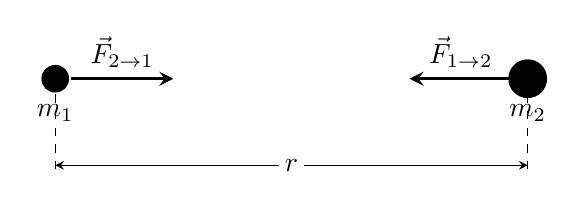
\begin{tikzpicture}[>=stealth, scale=1.0]
      
        % Massapunten
        \fill (-3,0) circle (5pt);
        \fill ( 3,0) circle (7pt);
      
        % Labels
        \node[below=6pt] at (-3,0) {$m_1$};
        \node[below=6pt] at ( 3,0) {$m_2$};
      
        % Gravitatiekrachten: naar elkaar gericht
        \draw[->, very thick] (-2.8,0) -- (-1.5,0)
            node[midway, above] {$\vec F_{2\to1}$};
      
        \draw[->, very thick] (2.8,0) -- (1.5,0)
            node[midway, above] {$\vec F_{1\to2}$};
      
        % Afstand tussen de massamiddelpunten
        \draw[<->] (-3,-1.1) -- (3,-1.1)
            node[midway, fill=white, inner sep=2pt] {$r$};
      
        % Hulplijnen
        \draw[dashed] (-3,-0.2) -- (-3,-1.25);
        \draw[dashed] ( 3,-0.2) -- ( 3,-1.25);
      
      \end{tikzpicture}
      \end{center}


We kunnen de formule lezen als een fysisch verhaal:

\[
\boxed{
F_g
\propto
m_1m_2
}
\]

en

\[
\boxed{
F_g
\propto
\frac{1}{r^2}.
}
\]


\FVDsubsection{Wat betekent $r$?}

Een belangrijke valkuil is de betekenis van de afstand $r$. Bij bolvormige hemellichamen gebruiken we de afstand tussen hun
\textbf{massamiddelpunten}.

Dus niet:

\begin{center}
de afstand tussen de oppervlakken,
\end{center}

maar:

\[
\boxed{
r=\text{afstand tussen de massamiddelpunten}.
}
\]


Wanneer een voorwerp zich op hoogte $h$ boven het aardoppervlak
bevindt, is de afstand tot het middelpunt van de aarde dus:

\begin{center}
      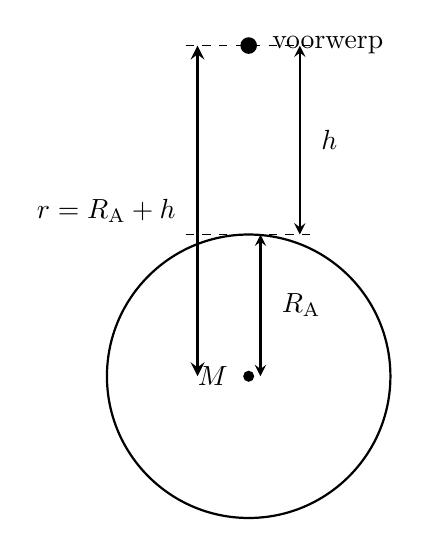
\begin{tikzpicture}[>=stealth, scale=1.0]
      
        % Aarde
        \coordinate (M) at (0,0);
        \draw[thick] (M) circle (1.8);
      
        % Middelpunt
        \fill (M) circle (2pt);
        \node[left=4pt] at (M) {$M$};
      
        % Voorwerp
        \coordinate (P) at (0,4.2);
        \fill (P) circle (3pt);
        \node[right=5pt] at (P) {voorwerp};
      
        % Straal van de aarde
        \draw[<->, thick] (0.15,0) -- (0.15,1.8)
          node[midway, right=4pt] {$R_{\mathrm A}$};
      
        % Hoogte boven het aardoppervlak
        \draw[<->, thick] (0.65,1.8) -- (0.65,4.2)
          node[midway, right=4pt] {$h$};
      
        % Volledige afstand tot het massamiddelpunt
        \draw[<->, very thick] (-0.65,0) -- (-0.65,4.2)
          node[midway, left=4pt] {$r=R_{\mathrm A}+h$};
      
        % Hulplijnen
        \draw[dashed] (-0.8,1.8) -- (0.8,1.8);
        \draw[dashed] (-0.8,4.2) -- (0.8,4.2);
      
      \end{tikzpicture}
      \end{center}

\[
\boxed{
r=R_\mathrm{A}+h.
}
\]

Niet:

\[
r=h.
\]


\begin{opmerking}

Voor bolsymmetrische massa's mogen we voor punten buiten de bol doen
alsof de volledige massa geconcentreerd is in het middelpunt.

Dat maakt de puntmassabenadering bijzonder bruikbaar voor planeten en
sterren.

\end{opmerking}


\begin{oefening}[De juiste afstand]{\oefB\ESS}

Een satelliet bevindt zich op hoogte $h$ boven het aardoppervlak.

Welke afstand moet in

\[
F_g=G\frac{Mm}{r^2}
\]

worden gebruikt?

Kies uit:

\[
r=h,
\qquad
r=R_\mathrm A,
\qquad
r=R_\mathrm A+h.
\]

Verklaar je keuze.


\begin{oplossing}

In de gravitatiewet is $r$ de afstand tussen de massamiddelpunten.

Een satelliet op hoogte $h$ boven het aardoppervlak bevindt zich daarom
op afstand

\[
\boxed{
r=R_\mathrm A+h
}
\]

van het aardmiddelpunt.

De keuze $r=h$ is fout omdat $h$ alleen vanaf het aardoppervlak wordt
gemeten. De keuze $r=R_\mathrm A$ geldt alleen aan het aardoppervlak.

\end{oplossing}

\end{oefening}


% ============================================================
% 4. EENHEDENCONTROLE
% ============================================================

\FVDsubsection{Eenheden als controle-instrument}

De eenheid van $G$ lijkt op het eerste gezicht ingewikkeld:

\[
[G]
=
\mathrm{\frac{N\,m^2}{kg^2}}.
\]

Maar precies die eenheid zorgt ervoor dat de gravitatiewet een kracht
oplevert.

Uit

\[
F_g
=
G\frac{m_1m_2}{r^2}
\]

volgt voor de eenheden:

\[
[F_g]
=
\mathrm{
\frac{N\,m^2}{kg^2}
\frac{kg\cdot kg}{m^2}
}.
\]

Dus:

\[
\boxed{
[F_g]=\mathrm N.
}
\]

Eenheden zijn daarom meer dan administratie. Ze vormen een eerste
controle op een fysische berekening.


% ============================================================
% 5. EERSTE BEREKENING
% ============================================================

\FVDsubsection{Hoe groot is gravitatie tussen gewone voorwerpen?}

De gravitatieconstante is zeer klein:

\[
G
=
6{,}674\times10^{-11}
\,
\mathrm{\frac{N\,m^2}{kg^2}}.
\]

Daarom is gravitatie tussen gewone voorwerpen meestal nauwelijks
merkbaar.


\begin{voorbeeld}[Twee leerlingen]

Twee leerlingen met massa's

\[
m_1=60\,\mathrm{kg}
\]

en

\[
m_2=70\,\mathrm{kg}
\]

bevinden zich met hun massamiddelpunten ongeveer

\[
r=1{,}0\,\mathrm m
\]

van elkaar.

De gravitatiekracht is

\[
F_g
=
G\frac{m_1m_2}{r^2}.
\]

Invullen geeft:

\[
F_g
=
6{,}674\times10^{-11}
\frac{60\cdot70}{1{,}0^2}.
\]

Dus:

\[
F_g
\approx
2{,}8\times10^{-7}\,\mathrm N.
\]
\begin{center}
      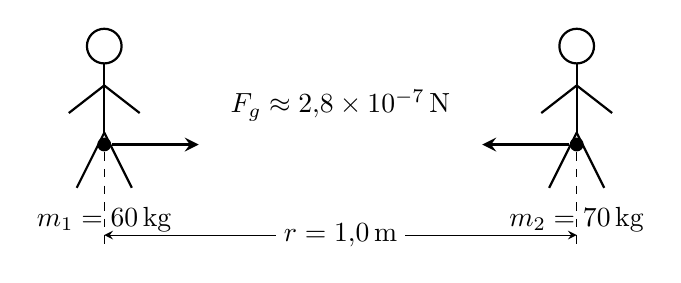
\begin{tikzpicture}[>=stealth, scale=1.0]
      
        % Leerlingen - schematisch
        \coordinate (A) at (-3,0);
        \coordinate (B) at ( 3,0);
      
        % Eenvoudige personen
        \draw[thick] (-3,1.25) circle (0.22);
        \draw[thick] (-3,1.03) -- (-3,0.15);
        \draw[thick] (-3,0.75) -- (-3.45,0.40);
        \draw[thick] (-3,0.75) -- (-2.55,0.40);
        \draw[thick] (-3,0.15) -- (-3.35,-0.55);
        \draw[thick] (-3,0.15) -- (-2.65,-0.55);
      
        \draw[thick] (3,1.25) circle (0.22);
        \draw[thick] (3,1.03) -- (3,0.15);
        \draw[thick] (3,0.75) -- (2.55,0.40);
        \draw[thick] (3,0.75) -- (3.45,0.40);
        \draw[thick] (3,0.15) -- (2.65,-0.55);
        \draw[thick] (3,0.15) -- (3.35,-0.55);
      
        % Massamiddelpunten
        \fill (A) circle (2.5pt);
        \fill (B) circle (2.5pt);
      
        % Massa's
        \node[below=19pt] at (A) {$m_1=60\,\mathrm{kg}$};
        \node[below=19pt] at (B) {$m_2=70\,\mathrm{kg}$};
      
        % Gravitatiekrachten
        \draw[->, very thick] (-2.9,0) -- (-1.8,0);
        \draw[->, very thick] ( 2.9,0) -- ( 1.8,0);
      
        \node[above=5pt] at (0,0)
          {$F_g\approx2{,}8\times10^{-7}\,\mathrm N$};
      
        % Afstand tussen massamiddelpunten
        \draw[<->] (-3,-1.15) -- (3,-1.15)
          node[midway, fill=white, inner sep=3pt]
          {$r=1{,}0\,\mathrm m$};
      
        % Hulplijnen
        \draw[dashed] (-3,-0.1) -- (-3,-1.3);
        \draw[dashed] ( 3,-0.1) -- ( 3,-1.3);
      
      \end{tikzpicture}
      \end{center}
Dat is extreem klein.

We merken de gravitatie tussen de leerlingen daarom niet.

De gravitatiekracht van de aarde op elke leerling is daarentegen wel
groot, omdat de aarde een enorme massa heeft.

\end{voorbeeld}


% ============================================================
% 6. PROBLEEMOPLOSSEN
% ============================================================

\FVDsubsection{Een gravitatieprobleem systematisch oplossen}

Bij een berekening is het verleidelijk onmiddellijk getallen in een
formule in te vullen.

Bij eenvoudige oefeningen lukt dat soms. Bij moeilijkere problemen
leidt het snel tot fouten.

Gebruik daarom een vaste aanpak.


\begin{center}
\[
\boxed{
\begin{array}{c}
\text{situatie begrijpen}
\\
\downarrow
\\
\text{schets maken}
\\
\downarrow
\\
\text{gegeven en gevraagd noteren}
\\
\downarrow
\\
\text{afstand }r\text{ correct bepalen}
\\
\downarrow
\\
\text{model kiezen}
\\
\downarrow
\\
\text{berekenen}
\\
\downarrow
\\
\text{eenheid en grootteorde controleren}
\\
\downarrow
\\
\text{antwoord fysisch interpreteren}
\end{array}
}
\]
\end{center}


Bij gravitatie is vooral de stap \(
\boxed{\text{bepaal }r}
\) belangrijk. Vraag jezelf steeds af:

\begin{center}
\textit{Welke afstand hoort werkelijk in de gravitatiewet?}
\end{center}


% ============================================================
% 7. OEFENING BASIS
% ============================================================

\begin{oefening}[Twee massa's]{\oefB\ESS}

Twee bolvormige voorwerpen hebben massa's

\[
m_1=5{,}0\,\mathrm{kg}
\qquad\text{en}\qquad
m_2=8{,}0\,\mathrm{kg}.
\]

Hun middelpunten bevinden zich op

\[
r=0{,}50\,\mathrm m
\]

van elkaar.

\begin{question}
Welke formule gebruik je om de gravitatiekracht te bepalen?
\end{question}

\begin{question}
Bereken de grootte van de gravitatiekracht.
\end{question}

\begin{question}
In welke richting werkt de kracht op $m_1$?
\end{question}

\begin{question}
In welke richting werkt de kracht op $m_2$?
\end{question}

\begin{oplossing}

      De grootte van de gravitatiekracht tussen twee massa's wordt gegeven
      door de algemene gravitatiewet:
      
      \[
      \boxed{
      F_g=G\frac{m_1m_2}{r^2}.
      }
      \]
      
      We vullen de gegeven waarden in:
      
      \[
      F_g
      =
      6{,}674\times10^{-11}
      \frac{5{,}0\cdot8{,}0}{(0{,}50)^2}.
      \]
      
      Hieruit volgt:
      
      \[
      \boxed{
      F_g\approx1{,}1\times10^{-8}\,\mathrm N.
      }
      \]
      
      De gravitatiekracht is een aantrekkingskracht. De kracht op $m_1$
      is daarom gericht naar $m_2$, terwijl de kracht op $m_2$ gericht is
      naar $m_1$.
      
      \begin{center}
      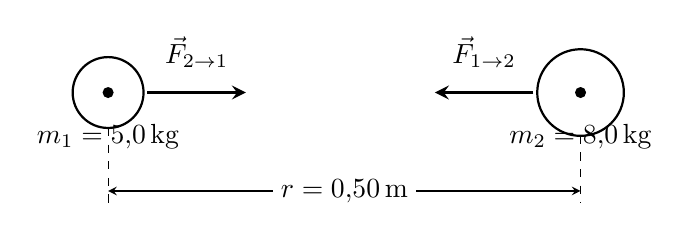
\begin{tikzpicture}[>=stealth]
      
        % Massamiddelpunten
        \coordinate (A) at (-3,0);
        \coordinate (B) at (3,0);
      
        % Bolvormige massa's
        \draw[thick] (A) circle (0.45);
        \draw[thick] (B) circle (0.55);
      
        % Massamiddelpunten
        \fill (A) circle (2pt);
        \fill (B) circle (2pt);
      
        % Labels
        \node[below=8pt] at (A) {$m_1=5{,}0\,\mathrm{kg}$};
        \node[below=8pt] at (B) {$m_2=8{,}0\,\mathrm{kg}$};
      
        % Kracht op m1 door m2
        \draw[->, very thick]
          (-2.5,0) -- (-1.25,0)
          node[midway, above=5pt] {$\vec F_{2\to1}$};
      
        % Kracht op m2 door m1
        \draw[->, very thick]
          (2.4,0) -- (1.15,0)
          node[midway, above=5pt] {$\vec F_{1\to2}$};
      
        % Afstand tussen de middelpunten
        \draw[<->]
          (-3,-1.25) -- (3,-1.25)
          node[midway, fill=white, inner sep=3pt]
          {$r=0{,}50\,\mathrm m$};
      
        % Hulplijnen
        \draw[dashed] (-3,-0.45) -- (-3,-1.40);
        \draw[dashed] ( 3,-0.55) -- ( 3,-1.40);
      
      \end{tikzpicture}
      \end{center}
      
      Beide krachten liggen op de verbindingslijn van de massamiddelpunten,
      zijn naar elkaar gericht en hebben dezelfde grootte:
      
      \[
      \left|\vec F_{2\to1}\right|
      =
      \left|\vec F_{1\to2}\right|
      \approx
      1{,}1\times10^{-8}\,\mathrm N.
      \]
      
      \end{oplossing}

\end{oefening}


\begin{oefening}[Twee bowlingballen]{\oefB}

Twee bowlingballen hebben elk een massa van

\[
7{,}0\,\mathrm{kg}.
\]

De afstand tussen hun massamiddelpunten is

\[
0{,}50\,\mathrm m.
\]

Bereken de gravitatiekracht die ze op elkaar uitoefenen.

Vergelijk de grootteorde met een kracht van $1\,\mathrm N$.


\begin{oplossing}

We gebruiken

\[
F_g=G\frac{m_1m_2}{r^2}.
\]

Met $m_1=m_2=7{,}0\,\mathrm{kg}$ en $r=0{,}50\,\mathrm m$:

\[
F_g
=
6{,}674\times10^{-11}
\frac{7{,}0\cdot7{,}0}{(0{,}50)^2}.
\]

Dus

\[
\boxed{
F_g\approx1{,}3\times10^{-8}\,\mathrm N.
}
\]

Vergeleken met $1\,\mathrm N$ is deze kracht ongeveer acht machten van
tien kleiner. De gravitatiekracht tussen voorwerpen met alledaagse
massa's is dus uiterst klein.

\end{oplossing}

\end{oefening}




\begin{oefening}[Satelliet op hoogte]{\oefB}

Een satelliet met massa

\[
m=500\,\mathrm{kg}
\]

bevindt zich op een hoogte

\[
h=400\,\mathrm{km}
\]

boven het aardoppervlak.

Gebruik

\[
M_\mathrm A=5{,}97\times10^{24}\,\mathrm{kg},
\qquad
R_\mathrm A=6{,}37\times10^6\,\mathrm m.
\]

\begin{enumerate}
  \item Zet de hoogte om naar meter.
  \item Bepaal de afstand $r$ van de satelliet tot het aardmiddelpunt.
  \item Bereken de grootte van de gravitatiekracht van de aarde op de
        satelliet.
  \item Leg uit waarom $h$ niet rechtstreeks als $r$ in de gravitatiewet
        mag worden ingevuld.
\end{enumerate}

\begin{oplossing}

\begin{enumerate}
  \item
  \[
  h=400\,\mathrm{km}=4{,}00\times10^5\,\mathrm m.
  \]

  \item De gravitatiewet gebruikt de afstand tot het massamiddelpunt:

  \[
  r=R_\mathrm A+h.
  \]

  Dus

  \[
  r
  =
  6{,}37\times10^6+4{,}00\times10^5
  =
  \boxed{6{,}77\times10^6\,\mathrm m}.
  \]

  \item We gebruiken

  \[
  F_g=G\frac{M_\mathrm A m}{r^2}.
  \]

  Invullen geeft

  \[
  F_g
  =
  6{,}674\times10^{-11}
  \frac{(5{,}97\times10^{24})(500)}
       {(6{,}77\times10^6)^2}.
  \]

  Daaruit volgt ongeveer

  \[
  \boxed{
  F_g\approx4{,}35\times10^3\,\mathrm N.
  }
  \]

  \item De hoogte $h$ wordt gemeten vanaf het aardoppervlak, terwijl
  $r$ in de gravitatiewet de afstand tussen de massamiddelpunten is.
  Daarom geldt

  \[
  \boxed{
  r=R_\mathrm A+h
  }
  \]

  en niet $r=h$.
\end{enumerate}

\end{oplossing}

\end{oefening}


% ============================================================
% 8. GRAVITATIE IS VECTORIEEL
% ============================================================

\FVDsection{De gravitatiekracht is een vector}

De formule

\[
F_g=G\frac{m_1m_2}{r^2}
\]

geeft alleen de \textbf{grootte} van de gravitatiekracht.
Maar een kracht is een vector. We moeten dus ook de
\textbf{richting} en \textbf{zin} kennen.

De gravitatiekracht werkt steeds langs de verbindingslijn tussen beide
massamiddelpunten en is steeds aantrekkend.

\begin{center}
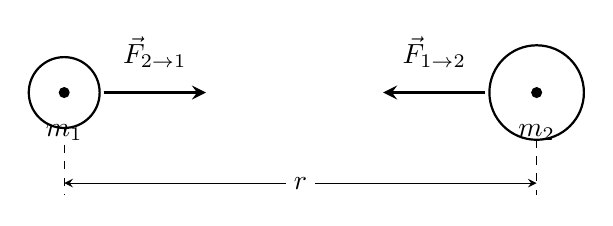
\begin{tikzpicture}[>=stealth]

  % Massamiddelpunten
  \coordinate (A) at (-3,0);
  \coordinate (B) at ( 3,0);

  % Massa's
  \draw[thick] (A) circle (0.45);
  \draw[thick] (B) circle (0.60);

  % Massamiddelpunten
  \fill (A) circle (2pt);
  \fill (B) circle (2pt);

  % Labels
  \node[below=8pt] at (A) {$m_1$};
  \node[below=8pt] at (B) {$m_2$};

  % Kracht op m1 door m2
  \draw[->, very thick]
    (-2.5,0) -- (-1.2,0)
    node[midway, above=5pt] {$\vec F_{2\to1}$};

  % Kracht op m2 door m1
  \draw[->, very thick]
    (2.35,0) -- (1.05,0)
    node[midway, above=5pt] {$\vec F_{1\to2}$};

  % Afstand tussen massamiddelpunten
  \draw[<->]
    (-3,-1.15) -- (3,-1.15)
    node[midway, fill=white, inner sep=3pt] {$r$};

  % Hulplijnen
  \draw[dashed] (-3,-0.45) -- (-3,-1.30);
  \draw[dashed] ( 3,-0.60) -- ( 3,-1.30);

\end{tikzpicture}
\end{center}

De kracht $\vec F_{2\to1}$ is de gravitatiekracht die $m_2$
uitoefent op $m_1$. Ze is gericht naar $m_2$.

De kracht $\vec F_{1\to2}$ is de gravitatiekracht die $m_1$
uitoefent op $m_2$. Ze is gericht naar $m_1$.

Beide krachten hebben dezelfde grootte:

\[
\left|\vec F_{2\to1}\right|
=
\left|\vec F_{1\to2}\right|
=
G\frac{m_1m_2}{r^2}.
\]

Ze hebben dezelfde richting, maar een tegengestelde zin. Daarom geldt
vectorieel:

\[
\boxed{
\vec F_{2\to1}=-\vec F_{1\to2}.
}
\]

Elke massa wordt dus naar de andere massa toe getrokken.

\begin{opmerking}

Bij gravitatie tussen gewone positieve massa's bestaat geen
gravitationele afstoting.

Dat wordt later een belangrijk verschil met elektrische krachten.

\end{opmerking}


% ============================================================
% 9. NEWTON III
% ============================================================

\FVDsection{Wie trekt het hardst?}

Stel dat de aarde een appel aantrekt. Welke kracht is groter? De kracht van de aarde op de appel? Of de kracht van de appel op de aarde?

Uit het vorige thema kennen we Newton III:

\[
\boxed{
\vec F_{A\rightarrow B}
=
-\vec F_{B\rightarrow A}.
}
\]

Dus:

\[
\boxed{
\vec F_{\mathrm{aarde}\rightarrow\mathrm{appel}}
=
-
\vec F_{\mathrm{appel}\rightarrow\mathrm{aarde}}.
}
\]

De krachten zijn exact even groot.

Dat lijkt misschien vreemd omdat de aarde zoveel zwaarder is.


\FVDsubsection{Waarom versnelt de appel dan zoveel meer?}

Newton II geeft:

\[
\vec a=\frac{\sum\vec F}{m}.
\]

De appel en de aarde ondervinden even grote interactiekrachten, maar hun
massa's verschillen enorm.

Voor de appel:

\[
a_\mathrm{appel}
=
\frac{F_g}{m_\mathrm{appel}}.
\]

Voor de aarde:

\[
a_\mathrm{aarde}
=
\frac{F_g}{M_\mathrm{aarde}}.
\]

Omdat

\[
M_\mathrm{aarde}
\gg
m_\mathrm{appel},
\]

geldt:

\[
a_\mathrm{aarde}
\ll
a_\mathrm{appel}.
\]


\begin{opmerking}

De aarde trekt niet harder aan de appel dan de appel aan de aarde.

De krachten zijn even groot.

Het verschil in bewegingsverandering ontstaat door het enorme verschil
in massa.

\end{opmerking}


\begin{oefening}[De aarde en jij]{\oefU\ESS}

Beschouw alleen de gravitatie-interactie tussen jou en de aarde.

Een leerling beweert:

\begin{center}
``De aarde trekt veel harder aan mij dan ik aan de aarde trek,
want de aarde heeft een veel grotere massa.''
\end{center}

Analyseer deze uitspraak.

Gebruik in je antwoord zowel Newton II als Newton III.

\begin{oplossing}

      De uitspraak is \textbf{onjuist}.
      
      Volgens \textbf{Newton III} oefenen de aarde en de leerling krachten
      op elkaar uit die even groot en tegengesteld gericht zijn:
      
      \[
      \boxed{
      \vec F_{\mathrm{aarde\to leerling}}
      =
      -\vec F_{\mathrm{leerling\to aarde}}
      }
      \]
      
      en dus
      
      \[
      \left|\vec F_{\mathrm{aarde\to leerling}}\right|
      =
      \left|\vec F_{\mathrm{leerling\to aarde}}\right|.
      \]
      
      De aarde trekt dus \textbf{niet harder} aan de leerling dan de
      leerling aan de aarde trekt.
      
      \begin{center}
      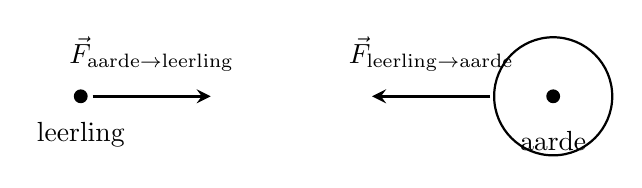
\begin{tikzpicture}[>=stealth]
      
        % Leerling
        \coordinate (L) at (-3,0);
        \fill (L) circle (2.5pt);
        \node[below=6pt] at (L) {leerling};
      
        % Aarde
        \coordinate (A) at (3,0);
        \draw[thick] (A) circle (0.75);
        \fill (A) circle (2.5pt);
        \node[below=9pt] at (A) {aarde};
      
        % Kracht op leerling
        \draw[->, very thick]
          (-2.85,0) -- (-1.35,0)
          node[midway, above=5pt]
          {$\vec F_{\mathrm{aarde\to leerling}}$};
      
        % Kracht op aarde
        \draw[->, very thick]
          (2.20,0) -- (0.70,0)
          node[midway, above=5pt]
          {$\vec F_{\mathrm{leerling\to aarde}}$};
      
      \end{tikzpicture}
      \end{center}
      
      Volgens \textbf{Newton II} geldt echter
      
      \[
      a=\frac{F}{m}.
      \]
      
      Hoewel beide krachten even groot zijn, zijn de massa's zeer
      verschillend.
      
      Voor de leerling geldt:
      
      \[
      a_{\mathrm{leerling}}
      =
      \frac{F_g}{m_{\mathrm{leerling}}},
      \]
      
      terwijl voor de aarde geldt:
      
      \[
      a_{\mathrm{aarde}}
      =
      \frac{F_g}{m_{\mathrm{aarde}}}.
      \]
      
      Omdat
      
      \[
      m_{\mathrm{aarde}}\gg m_{\mathrm{leerling}},
      \]
      
      volgt:
      
      \[
      \boxed{
      a_{\mathrm{aarde}}\ll a_{\mathrm{leerling}}.
      }
      \]
      
      De veel grotere massa van de aarde zorgt dus niet voor een grotere
      kracht op de leerling. Ze zorgt ervoor dat \textbf{dezelfde kracht
      een veel kleinere versnelling van de aarde veroorzaakt}.
      
      De leerling verwart dus \textbf{kracht} met \textbf{versnelling}.
      
      \end{oplossing}

\end{oefening}


\begin{oefening}[Gravitatie en Newton III]{\oefU}

De zon trekt de aarde aan.

\begin{enumerate}
  \item Oefent de aarde ook een gravitatiekracht uit op de zon?
  \item Vergelijk de groottes van beide krachten.
  \item Vergelijk kwalitatief de versnellingen van aarde en zon die door
        deze onderlinge interactie ontstaan.
  \item Verklaar waarom ``de zon trekt harder aan de aarde'' fysisch
        geen correcte formulering is.
\end{enumerate}


\begin{oplossing}

\begin{enumerate}
  \item Ja. De aarde oefent eveneens een gravitatiekracht uit op de zon.

  \item Volgens Newton III:

  \[
  \boxed{
  \vec F_{\mathrm{zon}\to\mathrm{aarde}}
  =
  -\vec F_{\mathrm{aarde}\to\mathrm{zon}}.
  }
  \]

  De krachten zijn dus even groot en tegengesteld gericht.

  \item Volgens Newton II geldt $a=F/m$. Omdat de zon veel meer massa
  heeft dan de aarde, veroorzaakt dezelfde interactiekracht een veel
  kleinere versnelling van de zon:

  \[
  \boxed{
  a_\mathrm{zon}<a_\mathrm{aarde}.
  }
  \]

  \item De uitspraak ``de zon trekt harder aan de aarde'' is fout omdat
  ze kracht en versnelling door elkaar haalt. De krachten zijn even
  groot; de versnellingen verschillen door het verschil in massa.
\end{enumerate}

\end{oplossing}

\end{oefening}


% ============================================================
% 10. INVLOED VAN DE MASSA
% ============================================================

\FVDsection{Hoe beïnvloeden de massa's de gravitatiekracht?}

De gravitatiekracht tussen twee massa's wordt gegeven door

\[
F_g
=
G\frac{m_1m_2}{r^2}.
\]

We onderzoeken eerst wat er gebeurt wanneer de afstand $r$ tussen
beide massamiddelpunten niet verandert.

Omdat $G$ en $r$ dan constant zijn, geldt

\[
\boxed{
F_g\propto m_1m_2.
}
\]

De gravitatiekracht is dus recht evenredig met het
\textbf{product van beide massa's}.


\FVDsubsection{Eén massa veranderen}

Stel dat alleen $m_1$ verdubbelt:

\[
m_1\longrightarrow 2m_1.
\]

Dan wordt

\[
F_g'
=
G\frac{(2m_1)m_2}{r^2}
=
2G\frac{m_1m_2}{r^2}.
\]

Dus

\[
\boxed{
F_g'=2F_g.
}
\]

Als één massa verdubbelt terwijl de andere massa en de afstand
onveranderd blijven, verdubbelt de gravitatiekracht.


\FVDsubsection{Beide massa's veranderen}

Stel nu dat beide massa's verdubbelen:

\[
m_1\longrightarrow2m_1,
\qquad
m_2\longrightarrow2m_2.
\]

Dan geldt

\[
F_g'
=
G\frac{(2m_1)(2m_2)}{r^2}
=
4G\frac{m_1m_2}{r^2}.
\]

Dus

\[
\boxed{
F_g'=4F_g.
}
\]

De factor $2$ van de eerste massa en de factor $2$ van de tweede
massa moeten dus met elkaar vermenigvuldigd worden:

\[
2\cdot2=4.
\]

\begin{center}
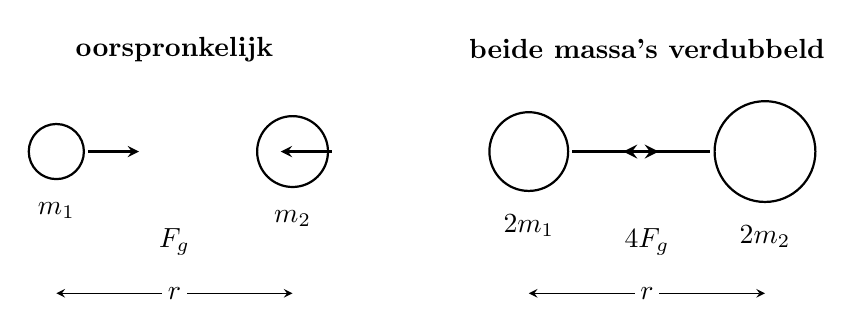
\begin{tikzpicture}[>=stealth]

  % -------------------------
  % Oorspronkelijke situatie
  % -------------------------
  \node at (-3,2.0) {\textbf{oorspronkelijk}};

  \draw[thick] (-4.5,0.7) circle (0.35);
  \draw[thick] (-1.5,0.7) circle (0.45);

  \node[below=5pt] at (-4.5,0.35) {$m_1$};
  \node[below=5pt] at (-1.5,0.25) {$m_2$};

  \draw[->, thick] (-4.1,0.7) -- (-3.45,0.7);
  \draw[->, thick] (-1.0,0.7) -- (-1.65,0.7);

  \node at (-3,-0.45) {$F_g$};

  % -------------------------
  % Nieuwe situatie
  % -------------------------
  \node at (3,2.0) {\textbf{beide massa's verdubbeld}};

  \draw[thick] (1.5,0.7) circle (0.50);
  \draw[thick] (4.5,0.7) circle (0.64);

  \node[below=5pt] at (1.5,0.20) {$2m_1$};
  \node[below=5pt] at (4.5,0.06) {$2m_2$};

  \draw[->, very thick] (2.05,0.7) -- (3.15,0.7);
  \draw[->, very thick] (3.80,0.7) -- (2.70,0.7);

  \node at (3,-0.45) {$4F_g$};

  % Zelfde afstand
  \draw[<->] (-4.5,-1.1) -- (-1.5,-1.1)
    node[midway, fill=white, inner sep=2pt] {$r$};

  \draw[<->] (1.5,-1.1) -- (4.5,-1.1)
    node[midway, fill=white, inner sep=2pt] {$r$};

\end{tikzpicture}
\end{center}

De afstand is in beide situaties dezelfde. De verandering van de
gravitatiekracht is dus uitsluitend het gevolg van de verandering
van de massa's.


\FVDsubsection{Een handige algemene regel}

We kunnen deze redenering veralgemenen.

Stel dat

\[
m_1\longrightarrow a\,m_1
\qquad\text{en}\qquad
m_2\longrightarrow b\,m_2,
\]

terwijl de afstand $r$ gelijk blijft.

Dan

\[
F_g'
=
G\frac{(a m_1)(b m_2)}{r^2}
=
ab\,G\frac{m_1m_2}{r^2}.
\]

Daarom geldt

\[
\boxed{
F_g'=ab\,F_g.
}
\]

De schaalfactor van de gravitatiekracht is dus het
\textbf{product van de schaalfactoren van beide massa's}.


\begin{oefening}[Redeneren zonder rekenen]{\oefB\ESS}

Een gravitatiekracht tussen twee massa's heeft oorspronkelijk
grootte $F$. De afstand tussen de massamiddelpunten blijft
onveranderd.

Bepaal telkens de nieuwe gravitatiekracht in functie van $F$.

\begin{enumerate}
  \item Alleen $m_1$ wordt driemaal zo groot.
  \item Beide massa's worden tweemaal zo groot.
  \item $m_1$ wordt gehalveerd en $m_2$ wordt verdubbeld.
  \item Beide massa's worden gehalveerd.
\end{enumerate}

Gebruik verhoudingen. Bereken de gravitatiekracht niet opnieuw vanaf
nul.

\end{oefening}


\begin{oplossing}

Bij constante afstand geldt

\[
F_g\propto m_1m_2.
\]

We hoeven dus alleen na te gaan met welke factor het product
$m_1m_2$ verandert.

\begin{enumerate}

  \item Alleen $m_1$ wordt driemaal zo groot.

  De schaalfactoren zijn $3$ en $1$. Dus

  \[
  F'=3\cdot1\cdot F.
  \]

  Bijgevolg:

  \[
  \boxed{F'=3F.}
  \]

  \item Beide massa's worden tweemaal zo groot.

  De schaalfactoren zijn $2$ en $2$. Dus

  \[
  F'=2\cdot2\cdot F.
  \]

  Bijgevolg:

  \[
  \boxed{F'=4F.}
  \]

  \item $m_1$ wordt gehalveerd en $m_2$ wordt verdubbeld.

  De schaalfactoren zijn $\frac12$ en $2$. Dus

  \[
  F'
  =
  \frac12\cdot2\cdot F
  =
  F.
  \]

  Bijgevolg:

  \[
  \boxed{F'=F.}
  \]

  De twee veranderingen heffen elkaar dus precies op.

  \item Beide massa's worden gehalveerd.

  De schaalfactoren zijn $\frac12$ en $\frac12$. Dus

  \[
  F'
  =
  \frac12\cdot\frac12\cdot F.
  \]

  Bijgevolg:

  \[
  \boxed{
  F'=\frac14F.
  }
  \]

\end{enumerate}

\end{oplossing}


% ============================================================
% 11. INVERSE-KWADRATENWET
% ============================================================

\FVDsection{Hoe beïnvloedt de afstand de gravitatiekracht?}

De gravitatiekracht tussen twee massa's wordt gegeven door

\[
F_g
=
G\frac{m_1m_2}{r^2}.
\]

We onderzoeken nu wat er gebeurt wanneer de massa's $m_1$ en $m_2$
onveranderd blijven en alleen de afstand $r$ verandert.

Omdat $G$, $m_1$ en $m_2$ dan constant zijn, geldt

\[
\boxed{
F_g\propto\frac{1}{r^2}.
}
\]

De gravitatiekracht is dus \textbf{omgekeerd evenredig met het
kwadraat van de afstand}.

We noemen dit een \textbf{inverse-kwadratenwet}.

\begin{opmerking}
De afstand $r$ is steeds de afstand tussen de
\textbf{massamiddelpunten} van beide voorwerpen.
\end{opmerking}


\FVDsubsection{Wat gebeurt er als de afstand verdubbelt?}

Stel dat de afstand tweemaal zo groot wordt:

\[
r\longrightarrow2r.
\]

Dan geldt

\[
F_g'
=
G\frac{m_1m_2}{(2r)^2}.
\]

Omdat

\[
(2r)^2=4r^2,
\]

vinden we

\[
F_g'
=
\frac14
G\frac{m_1m_2}{r^2}
=
\frac14F_g.
\]

Dus

\[
\boxed{
r\longrightarrow2r
\qquad\Longrightarrow\qquad
F_g\longrightarrow\frac14F_g.
}
\]

Een tweemaal zo grote afstand geeft dus een
\textbf{viermaal kleinere gravitatiekracht}.


\FVDsubsection{Een algemene regel}

We kunnen deze redenering veralgemenen.

Stel dat de afstand met een factor $k$ verandert:

\[
r\longrightarrow kr.
\]

Dan wordt de nieuwe gravitatiekracht

\[
F_g'
=
G\frac{m_1m_2}{(kr)^2}.
\]

Omdat

\[
(kr)^2=k^2r^2,
\]

volgt

\[
F_g'
=
\frac{1}{k^2}
G\frac{m_1m_2}{r^2}.
\]

Daarom geldt de algemene schaalregel

\[
\boxed{
F_g'=\frac{1}{k^2}F_g.
}
\]

De schaalfactor van de afstand moet dus eerst
\textbf{gekwadrateerd} en vervolgens \textbf{omgekeerd} worden.


\FVDsubsection{Enkele belangrijke gevallen}

Uit de algemene regel volgen onmiddellijk:

\[
\begin{array}{c|c|c}
\text{nieuwe afstand}
&
\text{schaalfactor van }r
&
\text{nieuwe gravitatiekracht}
\\
\hline
r       & 1             & F_g \\[2mm]
2r      & 2             & \dfrac14F_g \\[2mm]
3r      & 3             & \dfrac19F_g \\[2mm]
4r      & 4             & \dfrac1{16}F_g \\[2mm]
\dfrac r2 & \dfrac12    & 4F_g
\end{array}
\]

Merk vooral op dat de gravitatiekracht snel afneemt wanneer de
afstand groter wordt.

Omgekeerd neemt de gravitatiekracht snel toe wanneer de afstand
kleiner wordt.




\begin{oefening}[Afstand analyseren]{\oefU\ESS}

Twee massa's oefenen op afstand $r$ een gravitatiekracht $F$ op elkaar
uit.

Bepaal de nieuwe kracht wanneer de afstand:

\begin{enumerate}
  \item $2r$ wordt;
  \item $5r$ wordt;
  \item $r/3$ wordt;
  \item $0{,}8r$ wordt.
\end{enumerate}

Leg telkens uit hoe je tot je antwoord komt.

\begin{oplossing}

      Omdat de massa's niet veranderen, geldt
      
      \[
      F_g\propto\frac{1}{r^2}.
      \]
      
      Als de afstand verandert volgens
      
      \[
      r'=kr,
      \]
      
      dan verandert de gravitatiekracht volgens
      
      \[
      \boxed{
      F_g'=\frac{1}{k^2}F_g.
      }
      \]
      
      Aangezien de oorspronkelijke gravitatiekracht gelijk is aan $F$,
      kunnen we deze regel rechtstreeks toepassen.
      
      \begin{enumerate}
      
        \item De afstand wordt $2r$.
      
        De afstand wordt dus met een factor $2$ vermenigvuldigd:
      
        \[
        k=2.
        \]
      
        Daarom
      
        \[
        F_g'
        =
        \frac{1}{2^2}F
        =
        \boxed{\frac14F}.
        \]
      
        De afstand wordt tweemaal zo groot, waardoor de gravitatiekracht
        viermaal zo klein wordt.
      
      
        \item De afstand wordt $5r$.
      
        Nu is
      
        \[
        k=5.
        \]
      
        Daarom
      
        \[
        F_g'
        =
        \frac{1}{5^2}F
        =
        \boxed{\frac1{25}F}.
        \]
      
        De afstand wordt vijfmaal zo groot, waardoor de gravitatiekracht
        $25$ maal zo klein wordt.
      
      
        \item De afstand wordt $\dfrac r3$.
      
        De schaalfactor van de afstand is
      
        \[
        k=\frac13.
        \]
      
        Daarom
      
        \[
        F_g'
        =
        \frac{1}{\left(\frac13\right)^2}F
        =
        9F.
        \]
      
        Dus
      
        \[
        \boxed{F_g'=9F}.
        \]
      
        De afstand wordt driemaal zo klein, waardoor de gravitatiekracht
        negenmaal zo groot wordt.
      
      
        \item De afstand wordt $0{,}8r$.
      
        De schaalfactor van de afstand is
      
        \[
        k=0{,}8.
        \]
      
        Daarom
      
        \[
        F_g'
        =
        \frac{1}{(0{,}8)^2}F
        =
        \frac{1}{0{,}64}F
        =
        1{,}5625F.
        \]
      
        Dus
      
        \[
        \boxed{
        F_g'\approx1{,}56F.
        }
        \]
      
        De afstand neemt met $20\%$ af, maar de gravitatiekracht neemt
        daardoor niet met $20\%$ toe. Door de inverse-kwadratenwet wordt
        de kracht ongeveer $1{,}56$ maal zo groot.
      
      \end{enumerate}
      
      \end{oplossing}

\end{oefening}


\begin{oefening}[Combineren van veranderingen]{\oefU\ESS}

Twee massa's oefenen een gravitatiekracht $F$ op elkaar uit.

Daarna wordt:

\[
m_1'=2m_1,
\qquad
m_2'=3m_2,
\qquad
r'=2r.
\]

Bepaal zonder de oorspronkelijke waarden van de massa's of afstand te
kennen de verhouding

\[
\frac{F_g'}{F_g}.
\]

\begin{oplossing}

      Voor de oorspronkelijke situatie geldt
      
      \[
      F_g
      =
      G\frac{m_1m_2}{r^2}.
      \]
      
      Voor de nieuwe situatie geldt
      
      \[
      F_g'
      =
      G\frac{m_1'm_2'}{(r')^2}.
      \]
      
      We zoeken de verhouding van beide krachten:
      
      \[
      \frac{F_g'}{F_g}
      =
      \frac{
      G\dfrac{m_1'm_2'}{(r')^2}
      }{
      G\dfrac{m_1m_2}{r^2}
      }.
      \]
      
      Met
      
      \[
      m_1'=2m_1,
      \qquad
      m_2'=3m_2,
      \qquad
      r'=2r
      \]
      
      krijgen we
      
      \[
      \frac{F_g'}{F_g}
      =
      \frac{
      G\dfrac{(2m_1)(3m_2)}{(2r)^2}
      }{
      G\dfrac{m_1m_2}{r^2}
      }.
      \]
      
      De factoren $G$, $m_1$, $m_2$ en $r^2$ vallen weg:
      
      \[
      \frac{F_g'}{F_g}
      =
      \frac{2\cdot3}{2^2}.
      \]
      
      Dus
      
      \[
      \frac{F_g'}{F_g}
      =
      \frac64
      =
      \frac32.
      \]
      
      Bijgevolg
      
      \[
      \boxed{
      \frac{F_g'}{F_g}=\frac32
      }
      \]
      
      of, equivalent,
      
      \[
      \boxed{
      F_g'=1{,}5F_g.
      }
      \]
      
      We kunnen dit ook rechtstreeks met schaalfactoren begrijpen:
      
      \[
      \underbrace{2}_{m_1}
      \cdot
      \underbrace{3}_{m_2}
      \cdot
      \underbrace{\frac{1}{2^2}}_{r}
      =
      \frac32.
      \]
      
      De grotere massa's zouden de kracht samen met een factor $6$
      vergroten, terwijl de verdubbelde afstand de kracht met een factor
      $4$ verkleint. Het netto-effect is daarom een factor
      
      \[
      \boxed{\frac32}.
      \]
      
      \end{oplossing}

\end{oefening}


% ============================================================
% 12. VAN KRACHT NAAR VELD
% ============================================================

\FVDsection{Hoe weet een massa dat er een andere massa is?}

De gravitatiewet vertelt ons welke kracht twee massa's op elkaar
uitoefenen. Maar we kunnen de situatie ook op een andere manier beschrijven.

Neem de aarde.

Zelfs wanneer we nog geen tweede massa kiezen, kunnen we zeggen dat de
aarde de ruimte rondom zich fysisch beïnvloedt.

\begin{image}

\includegraphics{../images/Fysica/gravitatieveld.jpg}
\end{image}

Plaatsen we ergens in die ruimte een massa, dan ondervindt die een
gravitatiekracht. Om die invloed van de aarde op de ruimte te beschrijven voeren we het
begrip \textbf{gravitatieveld} in.


\begin{definitie}[Gravitatieveld]

Een massa veroorzaakt in de ruimte rondom zich een
\textbf{gravitatieveld}.

De gravitatieveldvector $\vec g$ in een punt wordt gedefinieerd als de
gravitatiekracht per eenheid massa die een kleine testmassa in dat punt
zou ondervinden:

\[
\boxed{
\vec g
=
\frac{\vec F_g}{m}.
}
\]

\end{definitie}


Dit is een belangrijke conceptuele overgang:

\[
\boxed{
\text{bronmassa}
\longrightarrow
\text{gravitatieveld}
\longrightarrow
\text{kracht op een massa}.
}
\]


% ============================================================
% 13. EENHEID VAN g
% ============================================================

\FVDsubsection{De eenheid van gravitatieveldsterkte}

Uit

\[
\vec g
=
\frac{\vec F_g}{m}
\]

volgt:

\[
[g]
=
\mathrm{\frac{N}{kg}}.
\]

Dus:

\[
\boxed{
[g]=\mathrm{N/kg}.
}
\]


Maar uit Newton II:

\[
\vec F=m\vec a
\]

volgt:

\[
\vec a=\frac{\vec F}{m}.
\]

Daarom is:

\[
1\,\mathrm{\frac{N}{kg}}
=
1\,\mathrm{\frac{m}{s^2}}.
\]

We kunnen $g$ dus op twee manieren interpreteren:

\[
\boxed{
g=\text{gravitatiekracht per kilogram}
}
\]

en

\[
\boxed{
g=\text{versnelling van een vrij vallende testmassa}.
}
\]


\begin{opmerking}

De twee eenheden

\[
\mathrm{N/kg}
\qquad\text{en}\qquad
\mathrm{m/s^2}
\]

zijn dimensioneel gelijkwaardig, maar benadrukken een andere
interpretatie.

Bij een \textbf{veld} gebruiken we vaak $\mathrm{N/kg}$.

Bij een \textbf{versnelling} gebruiken we meestal $\mathrm{m/s^2}$.

\end{opmerking}


% ============================================================
% 14. GRAVITATIEVELD VAN EEN MASSA
% ============================================================

\FVDsubsection{Het gravitatieveld van een bolvormige massa}

Beschouw een bolvormige bronmassa $M$. Op een afstand $r$ van het
massamiddelpunt plaatsen we een testmassa $m$.

De bronmassa oefent op de testmassa een gravitatiekracht uit met
grootte

\[
F_g
=
G\frac{Mm}{r^2}.
\]

Volgens de definitie van de gravitatieveldsterkte geldt

\[
g
=
\frac{F_g}{m}.
\]

Invullen geeft

\[
g
=
\frac{1}{m}
G\frac{Mm}{r^2}.
\]

De testmassa $m$ valt weg:

\[
\boxed{
g
=
G\frac{M}{r^2}.
}
\]

Dit resultaat is fundamenteel. De gravitatieveldsterkte wordt bepaald
door

\begin{itemize}
  \item de bronmassa $M$;
  \item de afstand $r$ tot het massamiddelpunt van de bronmassa.
\end{itemize}

Ze hangt niet af van de massa van het voorwerp waarmee we het veld
onderzoeken.


% ------------------------------------------------------------
% Figuur: bronmassa, testmassa en gravitatieveld
% ------------------------------------------------------------

\begin{center}
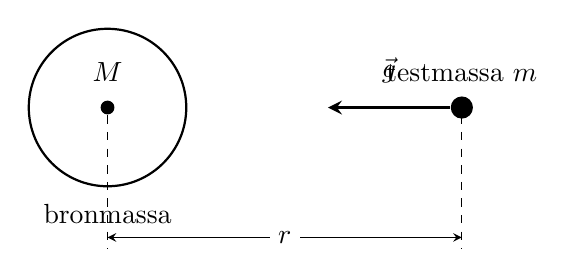
\begin{tikzpicture}[>=stealth]

  % Bronmassa
  \coordinate (M) at (0,0);
  \draw[thick] (M) circle (1.0);
  \fill (M) circle (2.5pt);

  \node at (0,0.45) {$M$};
  \node[below=3pt] at (0,-1.0) {bronmassa};

  % Testmassa
  \coordinate (P) at (4.5,0);
  \fill (P) circle (4pt);
  \node[above=6pt] at (P) {testmassa $m$};

  % g-vector
  \draw[->, very thick]
    (4.35,0) -- (2.8,0)
    node[midway, above=5pt] {$\vec g$};

  % afstand r
  \draw[<->]
    (0,-1.65) -- (4.5,-1.65)
    node[midway, fill=white, inner sep=3pt] {$r$};

  % hulplijnen
  \draw[dashed] (0,-0.1) -- (0,-1.8);
  \draw[dashed] (4.5,-0.1) -- (4.5,-1.8);

\end{tikzpicture}
\end{center}

De vector $\vec g$ wijst naar de bronmassa $M$.
Het gravitatieveld van een massa is immers aantrekkend.

Merk opnieuw op dat $r$ gemeten wordt vanaf het
\textbf{massamiddelpunt} van de bronmassa.


\FVDsubsection{Hoe verandert de veldsterkte met de afstand?}

Voor een vaste bronmassa $M$ geldt

\[
g
=
G\frac{M}{r^2}.
\]

Omdat $G$ en $M$ constant zijn, volgt

\[
\boxed{
g\propto\frac{1}{r^2}.
}
\]

De gravitatieveldsterkte volgt dus eveneens een
\textbf{inverse-kwadratenwet}.

Als de afstand bijvoorbeeld verdubbelt,

\[
r\longrightarrow2r,
\]

dan wordt

\[
g'
=
G\frac{M}{(2r)^2}
=
\frac14g.
\]

Dus

\[
\boxed{
r\longrightarrow2r
\qquad\Longrightarrow\qquad
g\longrightarrow\frac14g.
}
\]


% ------------------------------------------------------------
% Grafiek: g als functie van r
% ------------------------------------------------------------

\begin{center}
\begin{tikzpicture}
\begin{axis}[
    width=10cm,
    height=6.5cm,
    axis lines=left,
    xmin=0,
    xmax=4.3,
    ymin=0,
    ymax=4.5,
    xlabel={$\dfrac{r}{r_0}$},
    ylabel={$\dfrac{g}{g_0}$},
    xtick={0.5,1,2,3,4},
    ytick={0.25,1,2,3,4},
    domain=0.48:4.2,
    samples=150,
    clip=false
]

\addplot[thick] {1/x^2};

\addplot[only marks, mark=*]
coordinates {
    (0.5,4)
    (1,1)
    (2,0.25)
};

\node[anchor=south west] at (axis cs:0.5,4)
  {$\left(\frac12,4\right)$};

\node[anchor=south west] at (axis cs:1,1)
  {$(1,1)$};

\node[anchor=south west] at (axis cs:2,0.25)
  {$\left(2,\frac14\right)$};

\end{axis}
\end{tikzpicture}
\end{center}

De grafiek toont dat $g$ snel afneemt wanneer de afstand tot de
bronmassa groter wordt. Het verband is niet lineair.

Zo geldt bijvoorbeeld

\[
r=2r_0
\quad\Longrightarrow\quad
g=\frac14g_0,
\]

terwijl

\[
r=\frac12r_0
\quad\Longrightarrow\quad
g=4g_0.
\]


\begin{opmerking}

De formule

\[
\boxed{
g
=
G\frac{M}{r^2}
}
\]

geeft de \textbf{grootte} van de gravitatieveldsterkte die door de
bronmassa $M$ wordt veroorzaakt.

De richting van $\vec g$ is naar het massamiddelpunt van de
bronmassa gericht.

Een testmassa $m$ die zich in dat gravitatieveld bevindt, ondervindt
vervolgens een gravitatiekracht

\[
\boxed{
\vec F_g=m\vec g.
}
\]

De bronmassa bepaalt dus het gravitatieveld; een massa die in dat
veld wordt geplaatst, ondervindt daardoor een gravitatiekracht.

\end{opmerking}

\begin{oefening}[Gravitatieveld]{\oefB\ESS}

Een bolvormige planeet heeft massa $M$.

Een punt $P$ bevindt zich op afstand $r$ van het middelpunt.

\begin{enumerate}
  \item Schrijf de formule voor $g$ in $P$.
  \item Wat gebeurt er met $g$ wanneer $M$ verdubbelt?
  \item Wat gebeurt er met $g$ wanneer $r$ verdubbelt?
  \item Welke richting heeft $\vec g$?
\end{enumerate}


\begin{oplossing}

\begin{enumerate}
  \item
  \[
  \boxed{
  g=G\frac{M}{r^2}.
  }
  \]

  \item Bij vaste afstand geldt $g\propto M$. Als $M$ verdubbelt:
  \[
  \boxed{g'=2g.}
  \]

  \item Bij vaste bronmassa geldt $g\propto1/r^2$. Als $r$ verdubbelt:
  \[
  \boxed{g'=\frac14g.}
  \]

  \item De vector $\vec g$ wijst naar het massamiddelpunt van de
  bronmassa.
\end{enumerate}

\end{oplossing}

\end{oefening}


% ============================================================
% 15. WAAROM VALLEN MASSA'S EVEN SNEL?
% ============================================================

\FVDsubsection{Waarom hangt de valversnelling niet van de massa af?}

Een zwaarder voorwerp ondervindt een grotere gravitatiekracht:

\[
F_g
=
G\frac{Mm}{r^2}.
\]

Je zou daardoor kunnen verwachten dat een zwaarder voorwerp ook sneller
valt.

Maar volgens Newton II:

\[
a=\frac{F_g}{m}.
\]

Invullen geeft:

\[
a
=
\frac{1}{m}
G\frac{Mm}{r^2}.
\]

De massa $m$ van het vallende voorwerp valt weg:

\[
\boxed{
a
=
G\frac{M}{r^2}
=
g.
}
\]


\begin{center}
      \begin{tikzpicture}[>=stealth]
      
      % Titels
      \node at (-3,3.0) {\textbf{voorwerp 1}};
      \node at ( 3,3.0) {\textbf{voorwerp 2}};
      
      % Voorwerpen
      \draw[thick] (-3,2.1) circle (0.35);
      \draw[thick] ( 3,2.1) circle (0.50);
      
      \node at (-3,2.1) {$m$};
      \node at ( 3,2.1) {$2m$};
      
      % Gravitatiekrachten
      \draw[->, very thick]
        (-3,1.65) -- (-3,0.65)
        node[midway, left=5pt] {$F_g$};
      
      \draw[->, very thick]
        (3,1.50) -- (3,-0.50)
        node[midway, right=5pt] {$2F_g$};
      
      % Versnellingen
      \draw[->, thick]
        (-1.8,1.7) -- (-1.8,0.7)
        node[midway, right=4pt] {$\vec a=\vec g$};
      
      \draw[->, thick]
        (4.3,1.7) -- (4.3,0.7)
        node[midway, right=4pt] {$\vec a=\vec g$};
      
      % Vergelijking onderaan
      \node at (-3,-1.0)
        {$a=\dfrac{F_g}{m}=g$};
      
      \node at (3,-1.0)
        {$a=\dfrac{2F_g}{2m}=g$};
      
      \end{tikzpicture}
      \end{center}

      Het tweede voorwerp heeft tweemaal zoveel massa en ondervindt daarom
een tweemaal zo grote gravitatiekracht. Volgens Newton II moet die
grotere kracht echter ook een tweemaal zo grote massa versnellen:

\[
\frac{2F_g}{2m}
=
\frac{F_g}{m}.
\]

Daarom krijgen beide voorwerpen dezelfde valversnelling:

\[
\boxed{
a_1=a_2=g.
}
\]

Dus in hetzelfde gravitatieveld krijgen alle voorwerpen dezelfde
valversnelling, zolang andere krachten zoals luchtweerstand
verwaarloosbaar zijn.



\begin{oefening}[Hamer en veer]{\oefU\ESS}

Op de maan worden een hamer en een veer van dezelfde hoogte losgelaten.
Verwaarloos luchtweerstand.

\begin{enumerate}
  \item Welk voorwerp ondervindt de grootste gravitatiekracht?
  \item Welk voorwerp heeft de grootste valversnelling?
  \item Leg uit waarom je antwoorden op de vorige twee vragen niet met
        elkaar in tegenspraak zijn. Gebruik zowel de gravitatiewet als
        Newton II.
\end{enumerate}

\begin{oplossing}

      \begin{enumerate}
      
      \item
      De \textbf{hamer} ondervindt de grootste gravitatiekracht.
      
      Volgens de gravitatiewet geldt
      
      \[
      F_g
      =
      G\frac{Mm}{r^2}.
      \]
      
      De hamer en de veer bevinden zich praktisch op dezelfde afstand $r$
      van het middelpunt van de maan en de bronmassa $M$ is voor beide
      dezelfde.
      
      Daarom geldt
      
      \[
      F_g\propto m.
      \]
      
      Omdat de hamer een grotere massa heeft dan de veer, ondervindt de
      hamer dus een grotere gravitatiekracht.
      
      
      \item
      Beide voorwerpen hebben dezelfde valversnelling.
      
      Volgens Newton II geldt
      
      \[
      a=\frac{F_g}{m}.
      \]
      
      Met
      
      \[
      F_g
      =
      G\frac{Mm}{r^2}
      \]
      
      vinden we
      
      \[
      a
      =
      \frac{1}{m}
      G\frac{Mm}{r^2}
      =
      G\frac{M}{r^2}.
      \]
      
      De massa van het vallende voorwerp valt weg. Daarom geldt voor zowel
      de hamer als de veer
      
      \[
      \boxed{
      a=g_{\mathrm{maan}}.
      }
      \]
      
      
      \item
      Er is geen tegenspraak.
      
      De hamer heeft een grotere massa en ondervindt daardoor een grotere
      gravitatiekracht. Volgens Newton II moet die grotere kracht echter
      ook een grotere massa versnellen.
      
      Symbolisch:
      
      \[
      F_g\propto m
      \qquad\text{en}\qquad
      a=\frac{F_g}{m}.
      \]
      
      De grotere gravitatiekracht wordt dus precies gecompenseerd door de
      grotere massa:
      
      \[
      \boxed{
      a
      =
      G\frac{M}{r^2},
      }
      \]
      
      onafhankelijk van de massa van het vallende voorwerp.
      
      Omdat er op de maan praktisch geen atmosfeer is, speelt
      luchtweerstand geen betekenisvolle rol. De hamer en de veer vallen
      daarom met dezelfde valversnelling.
      
      \end{enumerate}
      
      \end{oplossing}


\end{oefening}

% ============================================================
% 16. g AAN HET AARDOPPERVLAK
% ============================================================

\FVDsubsection{Waar komt $9{,}81\,\mathrm{N/kg}$ vandaan?}

In eerdere fysica gebruikten we:

\[
g\approx9{,}81\,\mathrm{N/kg}.
\]

Nu kunnen we begrijpen waar die waarde vandaan komt.

Aan het aardoppervlak geldt ongeveer:

\[
r=R_\mathrm A.
\]

Dus:

\[
g
=
G\frac{M_\mathrm A}{R_\mathrm A^2}.
\]

Met ongeveer:

\[
M_\mathrm A
=
5{,}97\times10^{24}\,\mathrm{kg}
\]

en:

\[
R_\mathrm A
=
6{,}37\times10^6\,\mathrm m
\]

vinden we:

\[
g
=
6{,}674\times10^{-11}
\frac{5{,}97\times10^{24}}
{(6{,}37\times10^6)^2}.
\]

Dit geeft ongeveer:

\[
\boxed{
g\approx9{,}81\,\mathrm{N/kg}.
}
\]

De bekende waarde van $g$ is dus geen losstaande natuurconstante.

Ze volgt uit:

\[
\boxed{
G,\quad M_\mathrm A,\quad R_\mathrm A.
}
\]


\begin{oefening}[Een onbekende planeet]{\oefU\ESS}

Een planeet heeft tweemaal de massa van de aarde en tweemaal de straal
van de aarde:

\[
M_P=2M_\mathrm A,
\qquad
R_P=2R_\mathrm A.
\]

Bepaal de gravitatieveldsterkte aan het oppervlak van de planeet in
functie van $g_\mathrm A$.

Werk met verhoudingen en vermijd onnodige numerieke berekeningen.


\begin{oplossing}

Aan het oppervlak geldt

\[
g=G\frac{M}{R^2}.
\]

Daarom:

\[
\frac{g_P}{g_\mathrm A}
=
\frac{M_P}{M_\mathrm A}
\left(\frac{R_\mathrm A}{R_P}\right)^2.
\]

Met $M_P=2M_\mathrm A$ en $R_P=2R_\mathrm A$:

\[
\frac{g_P}{g_\mathrm A}
=
2\left(\frac12\right)^2
=
\frac12.
\]

Dus

\[
\boxed{
g_P=\frac12g_\mathrm A.
}
\]

De grotere massa versterkt het veld met factor $2$, maar de dubbele
straal verzwakt het veld met factor $2^2=4$. Netto blijft factor
$2/4=1/2$ over.

\end{oplossing}

\end{oefening}




\begin{oefening}[Een planeet ontdekken]{\oefG}

Astronomen ontdekken een bolvormige planeet.

Aan het oppervlak meten ze:

\[
g=12{,}0\,\mathrm{N/kg}.
\]

Uit astronomische waarnemingen bepalen ze de straal:

\[
R=8{,}0\times10^6\,\mathrm m.
\]

Gebruik

\[
g=G\frac{M}{R^2}
\]

om de massa van de planeet te bepalen.

Controleer vervolgens:

\begin{enumerate}
  \item de eenheid van je antwoord;
  \item de grootteorde;
  \item of een grotere straal bij dezelfde gemeten $g$ een grotere of
        kleinere planeetmassa zou vereisen.
\end{enumerate}


\begin{oplossing}

Uit

\[
g=G\frac{M}{R^2}
\]

volgt

\[
M=\frac{gR^2}{G}.
\]

Invullen geeft

\[
M
=
\frac{
12{,}0(8{,}0\times10^6)^2
}{
6{,}674\times10^{-11}
}.
\]

Dus

\[
\boxed{
M\approx1{,}15\times10^{25}\,\mathrm{kg}.
}
\]

Voor de eenheden:

\[
[M]
=
\frac{
\mathrm{N/kg}\,\mathrm{m^2}
}{
\mathrm{N\,m^2/kg^2}
}
=
\mathrm{kg}.
\]

De grootteorde is dus

\[
\boxed{10^{25}\,\mathrm{kg}},
\]

wat passend is voor een planeet.

Uit

\[
M=\frac{gR^2}{G}
\]

volgt bovendien dat bij dezelfde gemeten $g$ een grotere straal een
grotere massa vereist:

\[
\boxed{
M\propto R^2
\quad\text{bij constante }g.
}
\]

\end{oplossing}

\end{oefening}


% ============================================================
% 17. Fg = mg EN DE ALGEMENE WET
% ============================================================

\FVDsection{Hoe hangen $F_g=mg$ en de gravitatiewet samen?}

Nabij het aardoppervlak schrijven we:

\[
F_g=mg.
\]

De algemene gravitatiewet geeft:

\[
F_g
=
G\frac{M_\mathrm A m}{r^2}.
\]

Omdat:

\[
g
=
G\frac{M_\mathrm A}{r^2},
\]

volgt onmiddellijk:

\[
F_g=mg.
\]

Dus:

\[
\boxed{
F_g=mg
}
\]

is geen concurrerende wet.

Het is de praktische vorm van de gravitatiewet wanneer het lokale
gravitatieveld bekend is.


\begin{oefening}[Zelfde massa, kleinere planeet]{\oefU\ESS}

Een fictieve planeet heeft dezelfde massa als de aarde, maar slechts
de helft van de aardstraal.

\begin{enumerate}
  \item Hoe groot is $g$ aan het oppervlak ten opzichte van
        $g_\mathrm A$?
  \item Hoe groot is de gravitatiekracht op een astronaut van
        $80\,\mathrm{kg}$ ten opzichte van die op aarde?
  \item Verandert de massa van de astronaut?
\end{enumerate}


\begin{oplossing}

De planeet heeft $M_P=M_\mathrm A$ en
$R_P=\frac12R_\mathrm A$.

\begin{enumerate}
  \item
  \[
  \frac{g_P}{g_\mathrm A}
  =
  \frac{M_P}{M_\mathrm A}
  \left(\frac{R_\mathrm A}{R_P}\right)^2
  =
  1\cdot2^2=4.
  \]

  Dus

  \[
  \boxed{
  g_P=4g_\mathrm A.
  }
  \]

  \item Voor dezelfde astronaut geldt $F_g=mg$. Omdat zijn massa niet
  verandert en $g$ viermaal zo groot is:

  \[
  \boxed{
  F_{g,P}=4F_{g,\mathrm A}.
  }
  \]

  \item Nee. De massa blijft

  \[
  \boxed{
  m=80\,\mathrm{kg}.
  }
  \]
\end{enumerate}

\end{oplossing}

\end{oefening}


% ============================================================
% 18. MASSA, GRAVITATIEKRACHT EN GEWICHT
% ============================================================

\FVDsection{Massa, gravitatiekracht en gewicht}

In dagelijkse taal worden de woorden ``massa'' en ``gewicht'' vaak
door elkaar gebruikt. In fysica onderscheiden we drie begrippen.

\begin{description}

\item[Massa] is een eigenschap van een voorwerp. De massa wordt
uitgedrukt in

\[
\mathrm{kg}.
\]

\item[Gravitatiekracht] is de kracht waarmee een hemellichaam een
voorwerp aantrekt. In een gravitatieveld geldt

\[
\boxed{
\vec F_g=m\vec g.
}
\]

De gravitatiekracht wordt uitgedrukt in

\[
\mathrm N.
\]

\item[Gewicht] is de kracht die een voorwerp door de gravitatie op zijn
ondersteuning of ophanging uitoefent.

\end{description}

Massa, gravitatiekracht en gewicht zijn dus niet hetzelfde.

Een astronaut met massa

\[
80\,\mathrm{kg}
\]

heeft zowel op aarde als op de maan dezelfde massa. Omdat de
gravitatieveldsterkte op de maan kleiner is, is ook de gravitatiekracht
op de astronaut kleiner.

Het gewicht hangt bovendien af van de manier waarop het voorwerp wordt
ondersteund. Tijdens vrije val kan een voorwerp gravitatiekracht
ondervinden terwijl zijn gewicht nul is.

\begin{opmerking}

De formule

\[
F_g=mg
\]

berekent de \textbf{gravitatiekracht}. Ze mag dus niet zonder meer als
definitie van het gewicht worden gebruikt.

\end{opmerking}


\begin{oefening}[Aarde en maan]{\oefB\ESS}

Een astronaut heeft massa

\[
m=75\,\mathrm{kg}.
\]

Neem:

\[
g_\mathrm A=9{,}81\,\mathrm{N/kg}
\]

en:

\[
g_\mathrm M=1{,}62\,\mathrm{N/kg}.
\]

\begin{question}
Wat is de massa van de astronaut op aarde?
\end{question}

\begin{question}
Wat is zijn massa op de maan?
\end{question}

\begin{question}
Bereken de gravitatiekracht op de astronaut op aarde.
\end{question}

\begin{question}
Bereken de gravitatiekracht op de astronaut op de maan.
\end{question}

\begin{question}
Leg in woorden uit wat verandert en wat niet verandert.
\end{question}

\begin{oplossing}

      De massa van een voorwerp is onafhankelijk van de plaats waar het
      voorwerp zich bevindt. De gravitatiekracht berekenen we met
      
      \[
      \boxed{
      F_g=mg.
      }
      \]
      
      \begin{enumerate}
      
      \item
      De massa van de astronaut op aarde is
      
      \[
      \boxed{
      m=75\,\mathrm{kg}.
      }
      \]
      
      \item
      Ook op de maan blijft de massa van de astronaut
      
      \[
      \boxed{
      m=75\,\mathrm{kg}.
      }
      \]
      
      De massa verandert dus niet wanneer de astronaut van de aarde naar
      de maan gaat.
      
      
      \item
      Op aarde geldt
      
      \[
      F_{g,\mathrm A}
      =
      mg_{\mathrm A}.
      \]
      
      Invullen geeft
      
      \[
      F_{g,\mathrm A}
      =
      75\cdot9{,}81.
      \]
      
      Dus
      
      \[
      \boxed{
      F_{g,\mathrm A}
      \approx736\,\mathrm N.
      }
      \]
      
      
      \item
      Op de maan geldt
      
      \[
      F_{g,\mathrm M}
      =
      mg_{\mathrm M}.
      \]
      
      Invullen geeft
      
      \[
      F_{g,\mathrm M}
      =
      75\cdot1{,}62.
      \]
      
      Dus
      
      \[
      \boxed{
      F_{g,\mathrm M}
      \approx122\,\mathrm N.
      }
      \]
      
      
      \item
      De \textbf{massa} van de astronaut verandert niet:
      
      \[
      \boxed{
      m_{\mathrm A}=m_{\mathrm M}=75\,\mathrm{kg}.
      }
      \]
      
      De \textbf{gravitatieveldsterkte} is op de maan echter kleiner dan
      op aarde:
      
      \[
      g_{\mathrm M}<g_{\mathrm A}.
      \]
      
      Omdat
      
      \[
      F_g=mg,
      \]
      
      is ook de gravitatiekracht op de maan kleiner.
      
      De astronaut heeft dus overal dezelfde massa, maar ondervindt op de
      maan een kleinere gravitatiekracht dan op aarde.
      
      \end{enumerate}
      
      \end{oplossing}

\end{oefening}


% ============================================================
% 19. HOOGTE
% ============================================================

\FVDsection{Hoe verandert $g$ met de hoogte?}

Op hoogte $h$ boven het aardoppervlak is de afstand tot het middelpunt
van de aarde:

\[
r=R_\mathrm A+h.
\]

Daarom:

\[
\boxed{
g(h)
=
G\frac{M_\mathrm A}{(R_\mathrm A+h)^2}.
}
\]


Hieruit volgt onmiddellijk dat $g$ afneemt met de hoogte.

\begin{center}
      \begin{tikzpicture}
      \begin{axis}[
          width=10cm,
          height=6.5cm,
          axis lines=left,
          xmin=0,
          xmax=4.2,
          ymin=0,
          ymax=1.1,
          xlabel={$\dfrac{h}{R_{\mathrm A}}$},
          ylabel={$\dfrac{g}{g_0}$},
          xtick={0,1,2,3,4},
          ytick={0,0.25,0.5,0.75,1},
          domain=0:4,
          samples=150,
          clip=false
      ]
      
      % g/g0 = 1/(1+h/RA)^2
      \addplot[thick] {1/(1+x)^2};
      
      % Belangrijke punten
      \addplot[only marks, mark=*]
      coordinates {
          (0,1)
          (1,0.25)
      };
      
      \node[anchor=south west] at (axis cs:0,1)
          {$g=g_0$};
      
      \node[anchor=south west] at (axis cs:1,0.25)
          {$g=\dfrac14g_0$};
      
      % Hulplijnen voor h = RA
      \draw[dashed]
          (axis cs:1,0) -- (axis cs:1,0.25);
      
      \draw[dashed]
          (axis cs:0,0.25) -- (axis cs:1,0.25);
      
      \end{axis}
      \end{tikzpicture}
      \end{center}

      De grafiek toont dat de gravitatieveldsterkte afneemt wanneer de
      hoogte toeneemt. Die afname is niet lineair.
      
      Merk vooral op:
      
      \[
      h=R_{\mathrm A}
      \qquad\Longrightarrow\qquad
      r=2R_{\mathrm A}
      \qquad\Longrightarrow\qquad
      g=\frac14g_0.
      \]
      
      De inverse-kwadratenwet heeft betrekking op de afstand $r$ tot het
      \textbf{aardmiddelpunt}, niet rechtstreeks op de hoogte $h$ boven
      het aardoppervlak.


\begin{voorbeeld}[Op één aardstraal hoogte]

Stel dat een satelliet zich op hoogte

\[
h=R_\mathrm A
\]

boven het aardoppervlak bevindt.

Dan is zijn afstand tot het aardmiddelpunt:

\[
r=R_\mathrm A+h
=
2R_\mathrm A.
\]

Daarom:

\[
g
=
G\frac{M_\mathrm A}{(2R_\mathrm A)^2}.
\]

Dus:

\[
g
=
\frac14
G\frac{M_\mathrm A}{R_\mathrm A^2}.
\]

Bijgevolg:

\[
\boxed{
g=\frac14g_0.
}
\]

Let op: op een hoogte van één aardstraal is $g$ dus niet nul.

Het is nog steeds een kwart van de waarde aan het aardoppervlak.

\end{voorbeeld}


\begin{oefening}[Hoe hoog?]{\oefU\ESS}

Op welke hoogte boven het aardoppervlak is de gravitatieveldsterkte
gelijk aan

\[
\frac14g_0?
\]

Werk eerst symbolisch en leg duidelijk uit waarom de gezochte hoogte
niet gelijk is aan $2R_\mathrm A$.

\begin{oplossing}

      Aan het aardoppervlak geldt
      
      \[
      g_0
      =
      G\frac{M_\mathrm A}{R_\mathrm A^2}.
      \]
      
      Op een hoogte $h$ boven het aardoppervlak is de afstand tot het
      middelpunt van de aarde
      
      \[
      r=R_\mathrm A+h.
      \]
      
      Daarom geldt op die hoogte
      
      \[
      g(h)
      =
      G\frac{M_\mathrm A}{(R_\mathrm A+h)^2}.
      \]
      
      We zoeken de hoogte waarvoor
      
      \[
      g(h)=\frac14g_0.
      \]
      
      We stellen dus
      
      \[
      G\frac{M_\mathrm A}{(R_\mathrm A+h)^2}
      =
      \frac14
      G\frac{M_\mathrm A}{R_\mathrm A^2}.
      \]
      
      De factoren $G$ en $M_\mathrm A$ vallen weg:
      
      \[
      \frac{1}{(R_\mathrm A+h)^2}
      =
      \frac{1}{4R_\mathrm A^2}.
      \]
      
      Daaruit volgt
      
      \[
      (R_\mathrm A+h)^2
      =
      4R_\mathrm A^2.
      \]
      
      Omdat $R_\mathrm A+h$ een afstand is, nemen we de positieve
      wortel:
      
      \[
      R_\mathrm A+h
      =
      2R_\mathrm A.
      \]
      
      Dus
      
      \[
      h
      =
      2R_\mathrm A-R_\mathrm A.
      \]
      
      Bijgevolg:
      
      \[
      \boxed{
      h=R_\mathrm A.
      }
      \]
      
      De gezochte hoogte boven het aardoppervlak is dus één aardstraal.
      
      
      \textbf{Waarom is het antwoord niet $2R_\mathrm A$?}
      
      Om de gravitatieveldsterkte te verminderen tot
      
      \[
      \frac14g_0,
      \]
      
      moet de \textbf{afstand tot het middelpunt van de aarde} verdubbelen:
      
      \[
      r=2R_\mathrm A.
      \]
      
      Maar $r$ is niet de hoogte $h$. Er geldt
      
      \[
      r=R_\mathrm A+h.
      \]
      
      Daarom:
      
      \[
      2R_\mathrm A
      =
      R_\mathrm A+h
      \]
      
      en dus
      
      \[
      \boxed{
      h=R_\mathrm A.
      }
      \]
      
      \end{oplossing}

\end{oefening}


\begin{oefening}[Een fout analyseren]{\oefU}

Een leerling schrijft:

\[
g(h)
=
G\frac{M_\mathrm A}{h^2}.
\]

De leerling beweert dat deze formule de gravitatieveldsterkte op hoogte
$h$ boven het aardoppervlak geeft.

Analyseer de fout en geef de correcte formule.

Leg ook uit waarom de fout vooral voor kleine hoogtes tot absurde
resultaten leidt.


\begin{oplossing}

De fout is dat $h$ niet de afstand tot het aardmiddelpunt is.

Op hoogte $h$ boven het aardoppervlak geldt

\[
r=R_\mathrm A+h.
\]

De correcte formule is dus

\[
\boxed{
g(h)
=
G\frac{M_\mathrm A}{(R_\mathrm A+h)^2}.
}
\]

De fout wordt bijzonder duidelijk voor kleine hoogtes. Als bijvoorbeeld
$h$ naar nul nadert, zou de foutieve formule

\[
g(h)=G\frac{M_\mathrm A}{h^2}
\]

voorspellen dat $g$ onbeperkt groot wordt. In werkelijkheid nadert $g$
dan gewoon tot de eindige waarde aan het aardoppervlak:

\[
\boxed{
g_0=G\frac{M_\mathrm A}{R_\mathrm A^2}.
}
\]

\end{oplossing}

\end{oefening}


% ============================================================
% 20. VELDLIJNEN
% ============================================================

\FVDsection{Een onzichtbaar veld zichtbaar maken}

Een gravitatieveld kunnen we niet rechtstreeks zien. Om de structuur van een veld voor te stellen gebruiken we
\textbf{veldlijnen}.


\begin{definitie}[Gravitatieveldlijn]

Een gravitatieveldlijn is een denkbeeldige lijn waarvan de raaklijn in
elk punt de richting van de gravitatieveldvector aangeeft.

\end{definitie}

\begin{image}
      
\includegraphics{../images/Fysica/gravitatieveld1.png}
      
\includegraphics{../images/Fysica/gravitatieveld2.png}
\end{image}


Rond een bolvormige massa zijn de veldlijnen radiaal gericht naar het
middelpunt.

Dat komt doordat gravitatie aantrekkend is.


\begin{opmerking}

Uit een veldlijnenpatroon kunnen we twee soorten informatie halen:

\begin{itemize}
  \item de \textbf{richting en zin} van $\vec g$ worden aangegeven door
        de richting van de veldlijnen;
  \item waar de veldlijnen dichter bij elkaar liggen, stellen we een
        \textbf{sterker veld} voor.
\end{itemize}

\end{opmerking}


Omdat:

\[
g\propto\frac1{r^2},
\]

neemt de veldsterkte af naarmate we verder van de bronmassa komen.




\begin{oefening}[Veldlijnen lezen]{\oefB\ESS}

Beschouw het veldlijnenpatroon van een bolvormige massa.

\begin{enumerate}
  \item In welke zin wijzen de gravitatieveldlijnen?
  \item Waar is het gravitatieveld sterker: dicht bij de massa of verder
        weg?
  \item Hoe zie je dat kwalitatief aan het veldlijnenpatroon?
  \item Teken in een willekeurig punt op een veldlijn de richting en zin
        van $\vec g$.
\end{enumerate}

\begin{oplossing}

\begin{enumerate}
  \item De veldlijnen wijzen naar het massamiddelpunt, omdat gravitatie
        aantrekkend is.

  \item Het gravitatieveld is sterker dicht bij de massa.

  \item In de voorstelling liggen de veldlijnen daar dichter bij elkaar.
        Verder van de massa neemt de veldsterkte af.

  \item De vector $\vec g$ ligt raaklijnig aan de veldlijn in het gekozen
        punt en wijst in de zin van de veldlijn, dus naar de bronmassa.
\end{enumerate}

\end{oplossing}
\end{oefening}

% ============================================================
% 21. KRACHT OF VELD?
% ============================================================

\FVDsection{Gravitatiekracht of gravitatieveld?}

De begrippen worden gemakkelijk door elkaar gehaald.

Het verschil is fundamenteel.


\begin{center}
\[
\boxed{
\begin{array}{c|c}
\text{gravitatieveld} & \text{gravitatiekracht}\\
\hline
\vec g & \vec F_g\\[1mm]
\mathrm{N/kg} & \mathrm N\\[1mm]
\text{eigenschap van een punt in de ruimte}
&
\text{kracht op een gekozen massa}\\[1mm]
g=G\dfrac{M}{r^2}
&
F_g=G\dfrac{Mm}{r^2}\\[3mm]
&
\vec F_g=m\vec g
\end{array}
}
\]
\end{center}

\begin{center}
      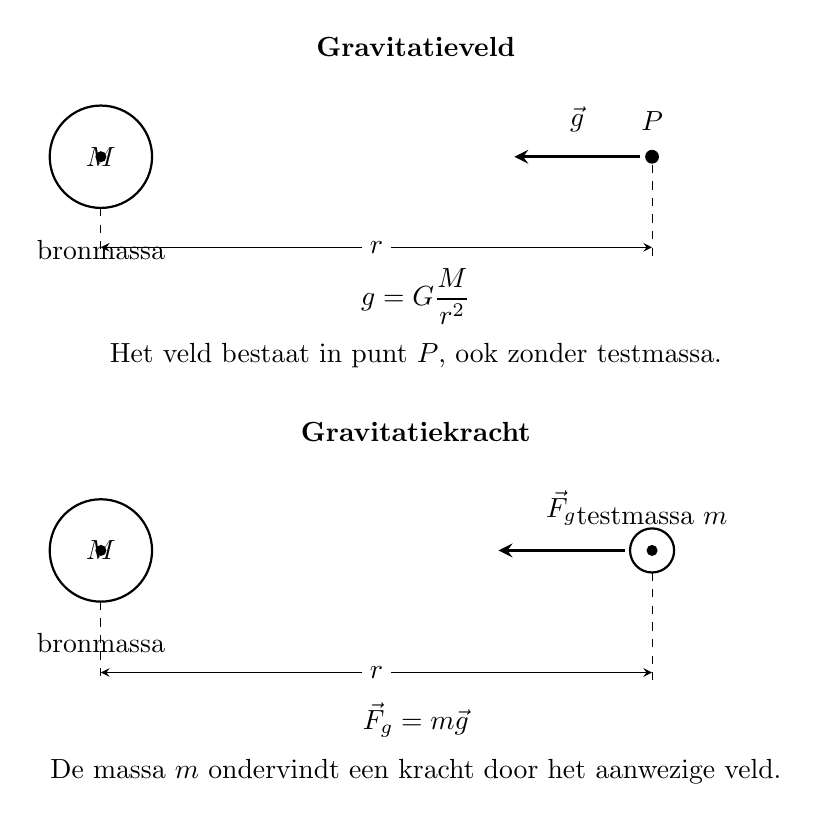
\begin{tikzpicture}[>=stealth, scale=1.0]
      
      % ============================================================
      % BOVEN: gravitatieveld
      % ============================================================
      
      \node[font=\bfseries] at (0,3.4)
        {Gravitatieveld};
      
      % Bronmassa
      \coordinate (M1) at (-4,2);
      \draw[thick] (M1) circle (0.65);
      \fill (M1) circle (2pt);
      \node at (M1) {$M$};
      \node[below=8pt] at (-4,1.35) {bronmassa};
      
      % Punt P
      \coordinate (P1) at (3,2);
      \fill (P1) circle (2.5pt);
      \node[above=6pt] at (P1) {$P$};
      
      % g-vector naar bronmassa
      \draw[->, very thick]
        (2.85,2) -- (1.25,2)
        node[midway, above=5pt] {$\vec g$};
      
      % Afstand
      \draw[<->]
        (-4,0.85) -- (3,0.85)
        node[midway, fill=white, inner sep=3pt] {$r$};
      
      \draw[dashed] (-4,1.35) -- (-4,0.70);
      \draw[dashed] ( 3,1.90) -- ( 3,0.70);
      
      \node[align=center] at (0,-0.05)
        {$\displaystyle g=G\frac{M}{r^2}$\\[2mm]
         Het veld bestaat in punt $P$, ook zonder testmassa.};
      
      
      % ============================================================
      % ONDER: gravitatiekracht
      % ============================================================
      
      \node[font=\bfseries] at (0,-1.5)
        {Gravitatiekracht};
      
      % Bronmassa
      \coordinate (M2) at (-4,-3);
      \draw[thick] (M2) circle (0.65);
      \fill (M2) circle (2pt);
      \node at (M2) {$M$};
      \node[below=8pt] at (-4,-3.65) {bronmassa};
      
      % Testmassa
      \coordinate (P2) at (3,-3);
      \draw[thick] (P2) circle (0.28);
      \fill (P2) circle (2pt);
      \node[above=6pt] at (P2) {testmassa $m$};
      
      % F-vector naar bronmassa
      \draw[->, very thick]
        (2.65,-3) -- (1.05,-3)
        node[midway, above=5pt] {$\vec F_g$};
      
      % Afstand
      \draw[<->]
        (-4,-4.55) -- (3,-4.55)
        node[midway, fill=white, inner sep=3pt] {$r$};
      
      \draw[dashed] (-4,-3.65) -- (-4,-4.70);
      \draw[dashed] ( 3,-3.28) -- ( 3,-4.70);
      
      \node[align=center] at (0,-5.45)
        {$\displaystyle \vec F_g=m\vec g$\\[2mm]
         De massa $m$ ondervindt een kracht door het aanwezige veld.};
      
      \end{tikzpicture}
      \end{center}

De bronmassa $M$ veroorzaakt een veld.

Een massa $m$ die in dat veld wordt geplaatst, ondervindt een kracht.

Dus:

\[
\boxed{
M
\longrightarrow
\vec g
\longrightarrow
\vec F_g\text{ op }m.
}
\]


\begin{oefening}[Kracht of veld?]{\oefB\ESS}

Geef telkens aan of de uitspraak betrekking heeft op $\vec F_g$ of
$\vec g$.

\begin{enumerate}
  \item De eenheid is $\mathrm N$.
  \item De eenheid is $\mathrm{N/kg}$.
  \item De grootheid beschrijft de invloed van de aarde in een punt in
        de ruimte.
  \item De grootheid hangt af van de massa van het voorwerp dat in het
        veld wordt geplaatst.
  \item De grootheid is nabij het aardoppervlak ongeveer
        $9{,}81\,\mathrm{N/kg}$.
\end{enumerate}

\begin{oplossing}

      We gebruiken het onderscheid:
      
      \[
      \boxed{
      \vec g
      =
      \text{gravitatieveldsterkte}
      }
      \qquad\text{en}\qquad
      \boxed{
      \vec F_g
      =
      \text{gravitatiekracht}.
      }
      \]
      
      \begin{enumerate}
      
        \item De eenheid is $\mathrm N$.
      
        De newton is de eenheid van kracht. De uitspraak heeft dus
        betrekking op
      
        \[
        \boxed{\vec F_g}.
        \]
      
      
        \item De eenheid is $\mathrm{N/kg}$.
      
        Dit is de eenheid van gravitatieveldsterkte. De uitspraak heeft dus
        betrekking op
      
        \[
        \boxed{\vec g}.
        \]
      
      
        \item De grootheid beschrijft de invloed van de aarde in een punt
        in de ruimte.
      
        Het gravitatieveld beschrijft de invloed van de aarde in een punt
        van de ruimte, ook wanneer daar geen testmassa aanwezig is.
      
        Dus:
      
        \[
        \boxed{\vec g}.
        \]
      
      
        \item De grootheid hangt af van de massa van het voorwerp dat in
        het veld wordt geplaatst.
      
        Voor een massa $m$ in een gravitatieveld geldt
      
        \[
        \vec F_g=m\vec g.
        \]
      
        De gravitatiekracht hangt dus af van $m$.
      
        Bijgevolg:
      
        \[
        \boxed{\vec F_g}.
        \]
      
      
        \item De grootheid is nabij het aardoppervlak ongeveer
        $9{,}81\,\mathrm{N/kg}$.
      
        Dit is de gravitatieveldsterkte nabij het aardoppervlak:
      
        \[
        \boxed{
        g\approx9{,}81\,\mathrm{N/kg}.
        }
        \]
      
        De uitspraak heeft dus betrekking op
      
        \[
        \boxed{\vec g}.
        \]
      
      \end{enumerate}
      
      Samengevat:
      
      \[
      \boxed{
      \begin{array}{c|ccccc}
      \text{uitspraak} & 1 & 2 & 3 & 4 & 5\\
      \hline
      \text{grootheid}
      & \vec F_g
      & \vec g
      & \vec g
      & \vec F_g
      & \vec g
      \end{array}
      }
      \]
      
      \end{oplossing}
\end{oefening}


% ============================================================
% 22. SUPERPOSITIE
% ============================================================

\FVDsection{Wanneer meerdere massa's aantrekken}

Tot nu toe bekeken we meestal één bronmassa. In werkelijkheid kan een voorwerp tegelijkertijd door verschillende
massa's worden aangetrokken.

De aarde ondervindt bijvoorbeeld gravitatie van de zon, de maan en alle andere hemellichamen.

Omdat kracht een vector is, geldt het superpositiebeginsel:

\[
\boxed{
\vec F_{g,\mathrm{res}}
=
\vec F_{g,1}
+
\vec F_{g,2}
+\cdots
}
\]


Voor gravitatievelden geldt analoog:

\[
\boxed{
\vec g_\mathrm{res}
=
\vec g_1
+
\vec g_2
+\cdots
}
\]


Dit is vectoriële optelling. We mogen dus niet zomaar de groottes van alle veldsterktes optellen.


\begin{image}
      
\includegraphics{../images/Fysica/gravitatieveld_aarde_maan.png}
\end{image}

\begin{voorbeeld}[Tussen twee gelijke massa's]

      Twee identieke bolvormige massa's $M$ bevinden zich op een afstand
      $d$ van elkaar.
      
      Beschouw het punt $P$ exact in het midden tussen beide massa's.
      De afstand van $P$ tot elke massa is dus
      
      \[
      \frac d2.
      \]
      
      Omdat beide bronmassa's even groot zijn en zich op dezelfde afstand
      van $P$ bevinden, veroorzaken ze daar gravitatievelden met dezelfde
      grootte.
      
      De veldvectoren zijn echter tegengesteld gericht.
      
      \begin{center}
      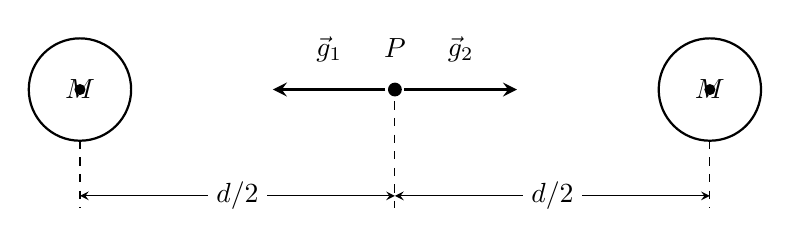
\begin{tikzpicture}[>=stealth]
      
        % Massa's
        \coordinate (M1) at (-4,0);
        \coordinate (M2) at ( 4,0);
        \coordinate (P)  at ( 0,0);
      
        \draw[thick] (M1) circle (0.65);
        \draw[thick] (M2) circle (0.65);
      
        \fill (M1) circle (2pt);
        \fill (M2) circle (2pt);
      
        \node at (M1) {$M$};
        \node at (M2) {$M$};
      
        % Middenpunt P
        \fill (P) circle (2.5pt);
        \node[above=8pt] at (P) {$P$};
      
        % Veldvector door linker massa
        \draw[->, very thick]
          (-0.12,0) -- (-1.55,0)
          node[midway, above=6pt] {$\vec g_1$};
      
        % Veldvector door rechter massa
        \draw[->, very thick]
          (0.12,0) -- (1.55,0)
          node[midway, above=6pt] {$\vec g_2$};
      
        % Afstanden
        \draw[<->]
          (-4,-1.35) -- (0,-1.35)
          node[midway, fill=white, inner sep=3pt] {$d/2$};
      
        \draw[<->]
          (0,-1.35) -- (4,-1.35)
          node[midway, fill=white, inner sep=3pt] {$d/2$};
      
        % Hulplijnen
        \draw[dashed] (-4,-0.65) -- (-4,-1.50);
        \draw[dashed] ( 0,-0.15) -- ( 0,-1.50);
        \draw[dashed] ( 4,-0.65) -- ( 4,-1.50);
      
      \end{tikzpicture}
      \end{center}
      
      Voor de linker massa wijst het gravitatieveld in $P$ naar links.
      Voor de rechter massa wijst het gravitatieveld in $P$ naar rechts.
      
      De grootte van beide veldsterktes is
      
      \[
      g_1
      =
      G\frac{M}{(d/2)^2}
      \qquad\text{en}\qquad
      g_2
      =
      G\frac{M}{(d/2)^2}.
      \]
      
      Dus
      
      \[
      g_1=g_2,
      \]
      
      maar de vectoren hebben een tegengestelde zin:
      
      \[
      \vec g_1=-\vec g_2.
      \]
      
      De resulterende gravitatieveldsterkte is de vectoriële som:
      
      \[
      \vec g_{\mathrm{res}}
      =
      \vec g_1+\vec g_2.
      \]
      
      Daarom:
      
      \[
      \boxed{
      \vec g_{\mathrm{res}}=\vec 0.
      }
      \]
      
      Er zijn in het midden dus wel twee gravitatievelden aanwezig, maar
      hun vectoriële som is nul.
      
      \end{voorbeeld}


\begin{oefening}[Nulveld]{\oefU\ESS}

Twee gelijke sterren bevinden zich op afstand $d$ van elkaar.

\begin{question}
Waar op de verbindingslijn ligt een punt waar het resulterende
gravitatieveld nul is?
\end{question}

\begin{question}
Betekent $\vec g_\mathrm{res}=\vec0$ dat geen van beide sterren daar
een gravitatieveld veroorzaakt?
\end{question}

\begin{question}
Wat verandert er wanneer de massa van één ster groter wordt?
Redeneer kwalitatief waar het nulpunt dan zal liggen.
\end{question}

\begin{oplossing}

      \begin{enumerate}
      
      \item
      Omdat beide sterren dezelfde massa hebben, veroorzaken ze in het
      midden tussen beide sterren gravitatievelden met dezelfde grootte.
      
      De afstand tot elke ster is daar
      
      \[
      \frac d2.
      \]
      
      De twee veldvectoren zijn tegengesteld gericht:
      
      \[
      \vec g_1=-\vec g_2.
      \]
      
      Daarom is hun vectoriële som nul:
      
      \[
      \boxed{
      \vec g_{\mathrm{res}}=\vec 0.
      }
      \]
      
      Het nulpunt ligt dus exact in het midden tussen beide sterren.
      
      
      \item
      Nee.
      
      Elke ster veroorzaakt afzonderlijk een gravitatieveld in dat punt:
      
      \[
      \vec g_1\neq\vec 0
      \qquad\text{en}\qquad
      \vec g_2\neq\vec 0.
      \]
      
      Omdat de sterren even zwaar zijn en het punt even ver van beide
      sterren ligt, zijn de groottes van beide veldsterktes gelijk:
      
      \[
      g_1=g_2.
      \]
      
      Hun zin is echter tegengesteld. Daarom heffen ze elkaar vectorieel op:
      
      \[
      \vec g_{\mathrm{res}}
      =
      \vec g_1+\vec g_2
      =
      \vec 0.
      \]
      
      Dus:
      
      \[
      \boxed{
      \vec g_{\mathrm{res}}=\vec 0
      \quad\text{betekent niet dat}\quad
      \vec g_1=\vec g_2=\vec 0.
      }
      \]
      
      
      \item
      Stel dat de linker ster een grotere massa krijgt:
      
      \[
      M_1>M_2.
      \]
      
      Op dezelfde afstand veroorzaakt de zwaardere ster een groter
      gravitatieveld, want
      
      \[
      g=G\frac{M}{r^2}.
      \]
      
      Het nulpunt kan daarom niet meer in het midden liggen. In het midden
      zou immers gelden
      
      \[
      g_1>g_2.
      \]
      
      Om de twee veldsterktes opnieuw even groot te maken, moeten we
      \textbf{verder van de zwaardere ster} en
      \textbf{dichter bij de lichtere ster} gaan.
      
      Het nulpunt verschuift dus naar de ster met de kleinste massa:
      
      \[
      \boxed{
      \text{het nulpunt ligt tussen beide sterren,
      maar dichter bij de lichtere ster.}
      }
      \]
      
      In het nulpunt geldt immers
      
      \[
      g_1=g_2,
      \]
      
      dus
      
      \[
      G\frac{M_1}{r_1^2}
      =
      G\frac{M_2}{r_2^2}.
      \]
      
      Wanneer $M_1>M_2$, moet bijgevolg ook
      
      \[
      r_1>r_2.
      \]
      
      Het nulpunt ligt dus verder van de zwaardere ster en dichter bij de
      lichtere ster.
      
      \end{enumerate}
      
      \end{oplossing}

\end{oefening}


\begin{oefening}[Waar ligt het nulpunt?]{\oefG}

Twee massa's $M$ en $4M$ bevinden zich op een afstand $d$ van elkaar.

Er bestaat tussen beide massa's een punt waar het resulterende
gravitatieveld nul is.

Noem de afstand van dit punt tot massa $M$ gelijk aan $x$.

\begin{enumerate}
  \item Maak een schets van beide gravitatieveldvectoren in het gezochte
        punt.
  \item Stel een vergelijking op voor $x$.
  \item Los de vergelijking op.
  \item Leg uit waarom het nulpunt dichter bij de kleinste massa ligt.
\end{enumerate}


\begin{oplossing}

Neem massa $M$ links en massa $4M$ rechts. Het gezochte punt ligt
tussen beide massa's, op afstand $x$ van $M$ en dus op afstand $d-x$
van $4M$.

In het nulpunt zijn de veldsterktes even groot en tegengesteld gericht:

\[
G\frac{M}{x^2}
=
G\frac{4M}{(d-x)^2}.
\]

Na schrappen van $G$ en $M$:

\[
\frac{1}{x^2}
=
\frac{4}{(d-x)^2}.
\]

Omdat de afstanden positief zijn:

\[
\frac1x=\frac{2}{d-x}.
\]

Dus

\[
d-x=2x,
\]

zodat

\[
\boxed{
x=\frac d3.
}
\]

Het nulpunt ligt dus op afstand $d/3$ van de massa $M$ en op afstand
$2d/3$ van de massa $4M$.

Dat het dichter bij de kleinste massa ligt, is logisch: om het zwakkere
veld van $M$ even groot te maken als het veld van $4M$, moet het punt
dichter bij $M$ liggen.

\end{oplossing}

\end{oefening}


\FVDsection{Waarom valt een satelliet niet op de aarde?}

Een satelliet in een baan rond de aarde wordt voortdurend door de
aarde aangetrokken. De gravitatiekracht is dus zeker niet verdwenen.

Een satelliet is eigenlijk voortdurend in \textbf{vrije val} naar de
aarde.

Toch bereikt hij het aardoppervlak niet. Terwijl de satelliet naar de
aarde valt, heeft hij immers ook een voldoende grote snelheid in een
richting langs het aardoppervlak. Daardoor blijft zijn baan voortdurend
rond de aarde afbuigen.

\begin{opmerking}
Een satelliet is dus niet ``buiten de zwaartekracht''.

Integendeel: de gravitatiekracht is juist verantwoordelijk voor de
voortdurende afbuiging van zijn beweging rond de aarde.
\end{opmerking}

\begin{center}
      \begin{tikzpicture}[>=stealth, scale=1.05]
      
      % ------------------------------------------------------------
      % Aarde
      % ------------------------------------------------------------
      \coordinate (O) at (0,0);
      
      \draw[thick] (O) circle (3);
      \fill (O) circle (2pt);
      \node[below right] at (O) {$M_{\mathrm A}$};
      
      % Eenvoudige continenten als visuele aanduiding
      \draw[thin]
        (-1.7,1.7) .. controls (-1.2,2.2) and (-0.5,2.0) .. (-0.3,1.5)
        .. controls (-0.7,1.1) and (-1.0,0.8) .. (-1.4,1.0);
      
      \draw[thin]
        (1.0,-0.7) .. controls (1.5,-0.4) and (2.0,-0.8) .. (1.8,-1.4)
        .. controls (1.4,-1.8) and (1.0,-1.5) .. (0.9,-1.1);
      
      % ------------------------------------------------------------
      % Kanon / lanceerpunt bovenaan
      % ------------------------------------------------------------
      \coordinate (L) at (0,3);
      
      \fill (L) circle (2.5pt);
      \node[left=5pt] at (L) {lanceerpunt};
      
      % Kanonloop
      \draw[very thick] (0,3.08) -- (0.75,3.08);
      \draw[thick] (0.05,2.95) rectangle (0.35,3.18);
      
      % Beginsnelheid
      \draw[->, very thick] (0.8,3.35) -- (2.1,3.35)
        node[midway, above] {$\vec v_0$};
      
      
      % ------------------------------------------------------------
      % Traject 1: kleine snelheid
      % ------------------------------------------------------------
      \draw[->, thick]
        (0.7,3.05)
        .. controls (1.35,3.00) and (1.75,2.65) ..
        (2.05,2.18);
      
      \node[anchor=west, align=left] at (2.15,2.55)
        {\small kleine snelheid};
      
      
      % ------------------------------------------------------------
      % Traject 2: grotere snelheid
      % ------------------------------------------------------------
      \draw[->, thick]
        (0.7,3.12)
        .. controls (2.0,3.15) and (3.25,2.25) ..
        (2.95,0.55);
      
      \node[anchor=west, align=left] at (3.15,1.45)
        {\small grotere snelheid};
      
      
      % ------------------------------------------------------------
      % Traject 3: satellietbaan
      % ------------------------------------------------------------
      \draw[thick, dashed] (O) circle (3.75);
      
      \draw[->, very thick]
        (0,3.75)
        arc[start angle=90,end angle=-35,radius=3.75];
      
      \node[anchor=west, align=left] at (3.6,-1.5)
        {\small voldoende grote snelheid:\\
         \small voortdurende vrije val};
      
      
      % ------------------------------------------------------------
      % Gravitatiekracht bij satelliet
      % ------------------------------------------------------------
      \coordinate (S) at ({3.75*cos(25)},{3.75*sin(25)});
      
      \fill (S) circle (2.5pt);
      
      \draw[->, very thick]
        (S) -- ($(S)!0.32!(O)$)
        node[pos=0.45, below right] {$\vec F_g$};
      
      
      % ------------------------------------------------------------
      % Onderschrift
      % ------------------------------------------------------------
      \node[align=center, text width=11cm] at (0,-4.35)
      {
      \small
      Hoe groter de horizontale beginsnelheid, hoe verder het voorwerp valt
      voordat het de aarde bereikt. Bij een geschikte snelheid blijft het
      voorwerp voortdurend naar de aarde vallen zonder het aardoppervlak te
      bereiken.
      };
      
      \end{tikzpicture}
      \end{center}


      Terwijl de satelliet naar de aarde valt, beweegt hij ook zijwaarts.
Bij een geschikte beginsnelheid kromt zijn baan voortdurend rond de
aarde: terwijl de satelliet valt, ``wijkt'' het aardoppervlak als het
ware voortdurend onder hem weg.







\begin{oefening}[Voortdurend vallen]{\oefU}

Een leerling zegt:

\begin{center}
``Een satelliet kan alleen rond de aarde blijven bewegen als daar bijna
geen zwaartekracht meer is.''
\end{center}

\begin{enumerate}
  \item Leg uit waarom deze uitspraak onjuist is.
  \item Wat zou er kwalitatief met de beweging van de satelliet gebeuren
        als de gravitatiekracht plots volledig verdween?
  \item Leg met de voorstelling van Newtons kanonskogel uit waarom een
        satelliet het aardoppervlak niet hoeft te bereiken terwijl hij
        toch voortdurend naar de aarde valt.
\end{enumerate}

\begin{oplossing}

\begin{enumerate}
  \item De uitspraak is onjuist. Een satelliet bevindt zich nog steeds in
        het gravitatieveld van de aarde en ondervindt dus een
        gravitatiekracht naar het aardmiddelpunt.

  \item Zonder gravitatie zou de beweging niet langer voortdurend naar de
        aarde afbuigen. De satelliet zou zijn gekromde baan dus niet
        blijven volgen.

  \item De satelliet heeft naast zijn valbeweging naar de aarde ook een
        voldoende grote zijwaartse snelheid. Terwijl hij valt, kromt het
        aardoppervlak als het ware onder hem weg. Daardoor blijft hij
        voortdurend vallen zonder het aardoppervlak te bereiken.
\end{enumerate}

\end{oplossing}
\end{oefening}


\end{document}